\documentclass[twoside]{book}

% Packages required by doxygen
\usepackage{fixltx2e}
\usepackage{calc}
\usepackage{doxygen}
\usepackage[export]{adjustbox} % also loads graphicx
\usepackage{graphicx}
\usepackage[utf8]{inputenc}
\usepackage{makeidx}
\usepackage{multicol}
\usepackage{multirow}
\PassOptionsToPackage{warn}{textcomp}
\usepackage{textcomp}
\usepackage[nointegrals]{wasysym}
\usepackage[table]{xcolor}

% Font selection
\usepackage[T1]{fontenc}
\usepackage[scaled=.90]{helvet}
\usepackage{courier}
\usepackage{amssymb}
\usepackage{sectsty}
\renewcommand{\familydefault}{\sfdefault}
\allsectionsfont{%
  \fontseries{bc}\selectfont%
  \color{darkgray}%
}
\renewcommand{\DoxyLabelFont}{%
  \fontseries{bc}\selectfont%
  \color{darkgray}%
}
\newcommand{\+}{\discretionary{\mbox{\scriptsize$\hookleftarrow$}}{}{}}

% Page & text layout
\usepackage{geometry}
\geometry{%
  a4paper,%
  top=2.5cm,%
  bottom=2.5cm,%
  left=2.5cm,%
  right=2.5cm%
}
\tolerance=750
\hfuzz=15pt
\hbadness=750
\setlength{\emergencystretch}{15pt}
\setlength{\parindent}{0cm}
\setlength{\parskip}{3ex plus 2ex minus 2ex}
\makeatletter
\renewcommand{\paragraph}{%
  \@startsection{paragraph}{4}{0ex}{-1.0ex}{1.0ex}{%
    \normalfont\normalsize\bfseries\SS@parafont%
  }%
}
\renewcommand{\subparagraph}{%
  \@startsection{subparagraph}{5}{0ex}{-1.0ex}{1.0ex}{%
    \normalfont\normalsize\bfseries\SS@subparafont%
  }%
}
\makeatother

% Headers & footers
\usepackage{fancyhdr}
\pagestyle{fancyplain}
\fancyhead[LE]{\fancyplain{}{\bfseries\thepage}}
\fancyhead[CE]{\fancyplain{}{}}
\fancyhead[RE]{\fancyplain{}{\bfseries\leftmark}}
\fancyhead[LO]{\fancyplain{}{\bfseries\rightmark}}
\fancyhead[CO]{\fancyplain{}{}}
\fancyhead[RO]{\fancyplain{}{\bfseries\thepage}}
\fancyfoot[LE]{\fancyplain{}{}}
\fancyfoot[CE]{\fancyplain{}{}}
\fancyfoot[RE]{\fancyplain{}{\bfseries\scriptsize Generated by Doxygen }}
\fancyfoot[LO]{\fancyplain{}{\bfseries\scriptsize Generated by Doxygen }}
\fancyfoot[CO]{\fancyplain{}{}}
\fancyfoot[RO]{\fancyplain{}{}}
\renewcommand{\footrulewidth}{0.4pt}
\renewcommand{\chaptermark}[1]{%
  \markboth{#1}{}%
}
\renewcommand{\sectionmark}[1]{%
  \markright{\thesection\ #1}%
}

% Indices & bibliography
\usepackage{natbib}
\usepackage[titles]{tocloft}
\setcounter{tocdepth}{3}
\setcounter{secnumdepth}{5}
\makeindex

% Hyperlinks (required, but should be loaded last)
\usepackage{ifpdf}
\ifpdf
  \usepackage[pdftex,pagebackref=true]{hyperref}
\else
  \usepackage[ps2pdf,pagebackref=true]{hyperref}
\fi
\hypersetup{%
  colorlinks=true,%
  linkcolor=blue,%
  citecolor=blue,%
  unicode%
}

% Custom commands
\newcommand{\clearemptydoublepage}{%
  \newpage{\pagestyle{empty}\cleardoublepage}%
}

\usepackage{caption}
\captionsetup{labelsep=space,justification=centering,font={bf},singlelinecheck=off,skip=4pt,position=top}

%===== C O N T E N T S =====

\begin{document}

% Titlepage & ToC
\hypersetup{pageanchor=false,
             bookmarksnumbered=true,
             pdfencoding=unicode
            }
\pagenumbering{alph}
\begin{titlepage}
\vspace*{7cm}
\begin{center}%
{\Large Rezerwacja }\\
\vspace*{1cm}
{\large Generated by Doxygen 1.8.14}\\
\end{center}
\end{titlepage}
\clearemptydoublepage
\pagenumbering{roman}
\tableofcontents
\clearemptydoublepage
\pagenumbering{arabic}
\hypersetup{pageanchor=true}

%--- Begin generated contents ---
\chapter{Namespace Index}
\section{Packages}
Here are the packages with brief descriptions (if available)\+:\begin{DoxyCompactList}
\item\contentsline{section}{\mbox{\hyperlink{namespace_engine}{Engine}} }{\pageref{namespace_engine}}{}
\item\contentsline{section}{\mbox{\hyperlink{namespace_silnik}{Silnik}} }{\pageref{namespace_silnik}}{}
\item\contentsline{section}{\mbox{\hyperlink{namespace_silnik_1_1_models}{Silnik.\+Models}} }{\pageref{namespace_silnik_1_1_models}}{}
\item\contentsline{section}{\mbox{\hyperlink{namespace_system_zarzadzania}{System\+Zarzadzania}} }{\pageref{namespace_system_zarzadzania}}{}
\item\contentsline{section}{\mbox{\hyperlink{namespace_system_zarzadzania_1_1_properties}{System\+Zarzadzania.\+Properties}} }{\pageref{namespace_system_zarzadzania_1_1_properties}}{}
\end{DoxyCompactList}

\chapter{Hierarchical Index}
\section{Class Hierarchy}
This inheritance list is sorted roughly, but not completely, alphabetically\+:\begin{DoxyCompactList}
\item Application\begin{DoxyCompactList}
\item \contentsline{section}{System\+Zarzadzania.\+App}{\pageref{class_system_zarzadzania_1_1_app}}{}
\item \contentsline{section}{System\+Zarzadzania.\+App}{\pageref{class_system_zarzadzania_1_1_app}}{}
\item \contentsline{section}{System\+Zarzadzania.\+App}{\pageref{class_system_zarzadzania_1_1_app}}{}
\end{DoxyCompactList}
\item \contentsline{section}{Silnik.\+Archiwum}{\pageref{class_silnik_1_1_archiwum}}{}
\item I\+Component\+Connector\begin{DoxyCompactList}
\item \contentsline{section}{System\+Zarzadzania.\+Main\+Window}{\pageref{class_system_zarzadzania_1_1_main_window}}{}
\item \contentsline{section}{System\+Zarzadzania.\+Main\+Window}{\pageref{class_system_zarzadzania_1_1_main_window}}{}
\end{DoxyCompactList}
\item I\+Notify\+Property\+Changed\begin{DoxyCompactList}
\item \contentsline{section}{Engine.\+Podstawowa\+Klasa\+Powiadomien}{\pageref{class_engine_1_1_podstawowa_klasa_powiadomien}}{}
\begin{DoxyCompactList}
\item \contentsline{section}{Silnik.\+Bilet}{\pageref{class_silnik_1_1_bilet}}{}
\item \contentsline{section}{Silnik.\+Klient}{\pageref{class_silnik_1_1_klient}}{}
\begin{DoxyCompactList}
\item \contentsline{section}{Silnik.\+Klient\+Indywidualny}{\pageref{class_silnik_1_1_klient_indywidualny}}{}
\item \contentsline{section}{Silnik.\+Posrednik}{\pageref{class_silnik_1_1_posrednik}}{}
\end{DoxyCompactList}
\item \contentsline{section}{Silnik.\+Lot}{\pageref{class_silnik_1_1_lot}}{}
\item \contentsline{section}{Silnik.\+Lotnisko}{\pageref{class_silnik_1_1_lotnisko}}{}
\item \contentsline{section}{Silnik.\+Models.\+Typ\+Samolotu}{\pageref{class_silnik_1_1_models_1_1_typ_samolotu}}{}
\item \contentsline{section}{Silnik.\+Samolot}{\pageref{class_silnik_1_1_samolot}}{}
\item \contentsline{section}{Silnik.\+Serwer\+Glowny}{\pageref{class_silnik_1_1_serwer_glowny}}{}
\item \contentsline{section}{Silnik.\+Trasa}{\pageref{class_silnik_1_1_trasa}}{}
\end{DoxyCompactList}
\end{DoxyCompactList}
\item Window\begin{DoxyCompactList}
\item \contentsline{section}{System\+Zarzadzania.\+Main\+Window}{\pageref{class_system_zarzadzania_1_1_main_window}}{}
\item \contentsline{section}{System\+Zarzadzania.\+Main\+Window}{\pageref{class_system_zarzadzania_1_1_main_window}}{}
\item \contentsline{section}{System\+Zarzadzania.\+Main\+Window}{\pageref{class_system_zarzadzania_1_1_main_window}}{}
\end{DoxyCompactList}
\end{DoxyCompactList}

\chapter{Class Index}
\section{Class List}
Here are the classes, structs, unions and interfaces with brief descriptions\+:\begin{DoxyCompactList}
\item\contentsline{section}{\mbox{\hyperlink{class_system_zarzadzania_1_1_app}{System\+Zarzadzania.\+App}} \\*Interaction logic for App.\+xaml }{\pageref{class_system_zarzadzania_1_1_app}}{}
\item\contentsline{section}{\mbox{\hyperlink{class_silnik_1_1_archiwum}{Silnik.\+Archiwum}} \\*The main \mbox{\hyperlink{class_silnik_1_1_archiwum}{Archiwum}} class. }{\pageref{class_silnik_1_1_archiwum}}{}
\item\contentsline{section}{\mbox{\hyperlink{class_silnik_1_1_bilet}{Silnik.\+Bilet}} \\*The main \mbox{\hyperlink{class_silnik_1_1_bilet}{Bilet}} class. Represents ticket and it values. }{\pageref{class_silnik_1_1_bilet}}{}
\item\contentsline{section}{\mbox{\hyperlink{class_silnik_1_1_klient}{Silnik.\+Klient}} \\*Main \mbox{\hyperlink{class_silnik_1_1_klient}{Klient}} class Represents base of clients representation. }{\pageref{class_silnik_1_1_klient}}{}
\item\contentsline{section}{\mbox{\hyperlink{class_silnik_1_1_klient_indywidualny}{Silnik.\+Klient\+Indywidualny}} \\*\mbox{\hyperlink{class_silnik_1_1_klient}{Klient}} class Represents individual clients. }{\pageref{class_silnik_1_1_klient_indywidualny}}{}
\item\contentsline{section}{\mbox{\hyperlink{class_silnik_1_1_lot}{Silnik.\+Lot}} \\*Base \mbox{\hyperlink{class_silnik_1_1_lot}{Lot}} class Represents flight. }{\pageref{class_silnik_1_1_lot}}{}
\item\contentsline{section}{\mbox{\hyperlink{class_silnik_1_1_lotnisko}{Silnik.\+Lotnisko}} \\*Base \mbox{\hyperlink{class_silnik_1_1_lotnisko}{Lotnisko}} class Represents airport. }{\pageref{class_silnik_1_1_lotnisko}}{}
\item\contentsline{section}{\mbox{\hyperlink{class_system_zarzadzania_1_1_main_window}{System\+Zarzadzania.\+Main\+Window}} \\*\mbox{\hyperlink{class_system_zarzadzania_1_1_main_window}{Main\+Window}} }{\pageref{class_system_zarzadzania_1_1_main_window}}{}
\item\contentsline{section}{\mbox{\hyperlink{class_engine_1_1_podstawowa_klasa_powiadomien}{Engine.\+Podstawowa\+Klasa\+Powiadomien}} }{\pageref{class_engine_1_1_podstawowa_klasa_powiadomien}}{}
\item\contentsline{section}{\mbox{\hyperlink{class_silnik_1_1_posrednik}{Silnik.\+Posrednik}} \\*\mbox{\hyperlink{class_silnik_1_1_posrednik}{Posrednik}} class Represents middleman. }{\pageref{class_silnik_1_1_posrednik}}{}
\item\contentsline{section}{\mbox{\hyperlink{class_silnik_1_1_samolot}{Silnik.\+Samolot}} }{\pageref{class_silnik_1_1_samolot}}{}
\item\contentsline{section}{\mbox{\hyperlink{class_silnik_1_1_serwer_glowny}{Silnik.\+Serwer\+Glowny}} }{\pageref{class_silnik_1_1_serwer_glowny}}{}
\item\contentsline{section}{\mbox{\hyperlink{class_silnik_1_1_trasa}{Silnik.\+Trasa}} }{\pageref{class_silnik_1_1_trasa}}{}
\item\contentsline{section}{\mbox{\hyperlink{class_silnik_1_1_models_1_1_typ_samolotu}{Silnik.\+Models.\+Typ\+Samolotu}} }{\pageref{class_silnik_1_1_models_1_1_typ_samolotu}}{}
\end{DoxyCompactList}

\chapter{Namespace Documentation}
\hypertarget{namespace_engine}{}\section{Engine Namespace Reference}
\label{namespace_engine}\index{Engine@{Engine}}
\subsection*{Classes}
\begin{DoxyCompactItemize}
\item 
class \mbox{\hyperlink{class_engine_1_1_podstawowa_klasa_powiadomien}{Podstawowa\+Klasa\+Powiadomien}}
\end{DoxyCompactItemize}

\hypertarget{namespace_silnik}{}\section{Silnik Namespace Reference}
\label{namespace_silnik}\index{Silnik@{Silnik}}
\subsection*{Namespaces}
\begin{DoxyCompactItemize}
\end{DoxyCompactItemize}
\subsection*{Classes}
\begin{DoxyCompactItemize}
\item 
class \mbox{\hyperlink{class_silnik_1_1_archiwum}{Archiwum}}
\begin{DoxyCompactList}\small\item\em The main \mbox{\hyperlink{class_silnik_1_1_archiwum}{Archiwum}} class. \end{DoxyCompactList}\item 
class \mbox{\hyperlink{class_silnik_1_1_bilet}{Bilet}}
\begin{DoxyCompactList}\small\item\em The main \mbox{\hyperlink{class_silnik_1_1_bilet}{Bilet}} class. Represents ticket and it values. \end{DoxyCompactList}\item 
class \mbox{\hyperlink{class_silnik_1_1_klient}{Klient}}
\begin{DoxyCompactList}\small\item\em Main \mbox{\hyperlink{class_silnik_1_1_klient}{Klient}} class Represents base of clients representation. \end{DoxyCompactList}\item 
class \mbox{\hyperlink{class_silnik_1_1_klient_indywidualny}{Klient\+Indywidualny}}
\begin{DoxyCompactList}\small\item\em \mbox{\hyperlink{class_silnik_1_1_klient}{Klient}} class Represents individual clients. \end{DoxyCompactList}\item 
class \mbox{\hyperlink{class_silnik_1_1_lot}{Lot}}
\begin{DoxyCompactList}\small\item\em Base \mbox{\hyperlink{class_silnik_1_1_lot}{Lot}} class Represents flight. \end{DoxyCompactList}\item 
class \mbox{\hyperlink{class_silnik_1_1_lotnisko}{Lotnisko}}
\begin{DoxyCompactList}\small\item\em Base \mbox{\hyperlink{class_silnik_1_1_lotnisko}{Lotnisko}} class Represents airport. \end{DoxyCompactList}\item 
class \mbox{\hyperlink{class_silnik_1_1_posrednik}{Posrednik}}
\begin{DoxyCompactList}\small\item\em \mbox{\hyperlink{class_silnik_1_1_posrednik}{Posrednik}} class Represents middleman. \end{DoxyCompactList}\item 
class \mbox{\hyperlink{class_silnik_1_1_samolot}{Samolot}}
\item 
class \mbox{\hyperlink{class_silnik_1_1_serwer_glowny}{Serwer\+Glowny}}
\item 
class \mbox{\hyperlink{class_silnik_1_1_trasa}{Trasa}}
\end{DoxyCompactItemize}

\hypertarget{namespace_silnik_1_1_models}{}\section{Silnik.\+Models Namespace Reference}
\label{namespace_silnik_1_1_models}\index{Silnik.\+Models@{Silnik.\+Models}}
\subsection*{Classes}
\begin{DoxyCompactItemize}
\item 
class \mbox{\hyperlink{class_silnik_1_1_models_1_1_typ_samolotu}{Typ\+Samolotu}}
\end{DoxyCompactItemize}

\hypertarget{namespace_system_zarzadzania}{}\section{System\+Zarzadzania Namespace Reference}
\label{namespace_system_zarzadzania}\index{System\+Zarzadzania@{System\+Zarzadzania}}
\subsection*{Namespaces}
\begin{DoxyCompactItemize}
\end{DoxyCompactItemize}
\subsection*{Classes}
\begin{DoxyCompactItemize}
\item 
class \mbox{\hyperlink{class_system_zarzadzania_1_1_app}{App}}
\begin{DoxyCompactList}\small\item\em Interaction logic for App.\+xaml \end{DoxyCompactList}\item 
class \mbox{\hyperlink{class_system_zarzadzania_1_1_main_window}{Main\+Window}}
\begin{DoxyCompactList}\small\item\em \mbox{\hyperlink{class_system_zarzadzania_1_1_main_window}{Main\+Window}} \end{DoxyCompactList}\end{DoxyCompactItemize}

\hypertarget{namespace_system_zarzadzania_1_1_properties}{}\section{System\+Zarzadzania.\+Properties Namespace Reference}
\label{namespace_system_zarzadzania_1_1_properties}\index{System\+Zarzadzania.\+Properties@{System\+Zarzadzania.\+Properties}}
\subsection*{Classes}
\begin{DoxyCompactItemize}
\item 
class {\bfseries Resources}
\begin{DoxyCompactList}\small\item\em A strongly-\/typed resource class, for looking up localized strings, etc. \end{DoxyCompactList}\item 
class {\bfseries Settings}
\end{DoxyCompactItemize}

\chapter{Class Documentation}
\hypertarget{class_system_zarzadzania_1_1_app}{}\section{System\+Zarzadzania.\+App Class Reference}
\label{class_system_zarzadzania_1_1_app}\index{System\+Zarzadzania.\+App@{System\+Zarzadzania.\+App}}


Interaction logic for App.\+xaml  


Inheritance diagram for System\+Zarzadzania.\+App\+:\begin{figure}[H]
\begin{center}
\leavevmode
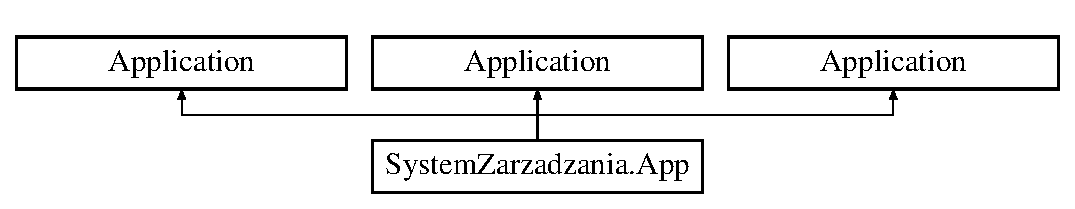
\includegraphics[height=2.000000cm]{class_system_zarzadzania_1_1_app}
\end{center}
\end{figure}
\subsection*{Public Member Functions}
\begin{DoxyCompactItemize}
\item 
void \mbox{\hyperlink{class_system_zarzadzania_1_1_app_ac1f3db202350dcc6d30936a6ddf65a86}{Initialize\+Component}} ()
\begin{DoxyCompactList}\small\item\em Initialize\+Component \end{DoxyCompactList}\item 
void \mbox{\hyperlink{class_system_zarzadzania_1_1_app_ac1f3db202350dcc6d30936a6ddf65a86}{Initialize\+Component}} ()
\begin{DoxyCompactList}\small\item\em Initialize\+Component \end{DoxyCompactList}\end{DoxyCompactItemize}
\subsection*{Static Public Member Functions}
\begin{DoxyCompactItemize}
\item 
static void \mbox{\hyperlink{class_system_zarzadzania_1_1_app_afc35a78a384092bf9baa0d4c310c2ebe}{Main}} ()
\begin{DoxyCompactList}\small\item\em Application Entry Point. \end{DoxyCompactList}\item 
static void \mbox{\hyperlink{class_system_zarzadzania_1_1_app_afc35a78a384092bf9baa0d4c310c2ebe}{Main}} ()
\begin{DoxyCompactList}\small\item\em Application Entry Point. \end{DoxyCompactList}\end{DoxyCompactItemize}


\subsection{Detailed Description}
Interaction logic for App.\+xaml 

\mbox{\hyperlink{class_system_zarzadzania_1_1_app}{App}} 

\subsection{Member Function Documentation}
\mbox{\Hypertarget{class_system_zarzadzania_1_1_app_ac1f3db202350dcc6d30936a6ddf65a86}\label{class_system_zarzadzania_1_1_app_ac1f3db202350dcc6d30936a6ddf65a86}} 
\index{System\+Zarzadzania\+::\+App@{System\+Zarzadzania\+::\+App}!Initialize\+Component@{Initialize\+Component}}
\index{Initialize\+Component@{Initialize\+Component}!System\+Zarzadzania\+::\+App@{System\+Zarzadzania\+::\+App}}
\subsubsection{\texorpdfstring{Initialize\+Component()}{InitializeComponent()}\hspace{0.1cm}{\footnotesize\ttfamily [1/2]}}
{\footnotesize\ttfamily void System\+Zarzadzania.\+App.\+Initialize\+Component (\begin{DoxyParamCaption}{ }\end{DoxyParamCaption})}



Initialize\+Component 

\mbox{\Hypertarget{class_system_zarzadzania_1_1_app_ac1f3db202350dcc6d30936a6ddf65a86}\label{class_system_zarzadzania_1_1_app_ac1f3db202350dcc6d30936a6ddf65a86}} 
\index{System\+Zarzadzania\+::\+App@{System\+Zarzadzania\+::\+App}!Initialize\+Component@{Initialize\+Component}}
\index{Initialize\+Component@{Initialize\+Component}!System\+Zarzadzania\+::\+App@{System\+Zarzadzania\+::\+App}}
\subsubsection{\texorpdfstring{Initialize\+Component()}{InitializeComponent()}\hspace{0.1cm}{\footnotesize\ttfamily [2/2]}}
{\footnotesize\ttfamily void System\+Zarzadzania.\+App.\+Initialize\+Component (\begin{DoxyParamCaption}{ }\end{DoxyParamCaption})}



Initialize\+Component 

\mbox{\Hypertarget{class_system_zarzadzania_1_1_app_afc35a78a384092bf9baa0d4c310c2ebe}\label{class_system_zarzadzania_1_1_app_afc35a78a384092bf9baa0d4c310c2ebe}} 
\index{System\+Zarzadzania\+::\+App@{System\+Zarzadzania\+::\+App}!Main@{Main}}
\index{Main@{Main}!System\+Zarzadzania\+::\+App@{System\+Zarzadzania\+::\+App}}
\subsubsection{\texorpdfstring{Main()}{Main()}\hspace{0.1cm}{\footnotesize\ttfamily [1/2]}}
{\footnotesize\ttfamily static void System\+Zarzadzania.\+App.\+Main (\begin{DoxyParamCaption}{ }\end{DoxyParamCaption})\hspace{0.3cm}{\ttfamily [static]}}



Application Entry Point. 

\mbox{\Hypertarget{class_system_zarzadzania_1_1_app_afc35a78a384092bf9baa0d4c310c2ebe}\label{class_system_zarzadzania_1_1_app_afc35a78a384092bf9baa0d4c310c2ebe}} 
\index{System\+Zarzadzania\+::\+App@{System\+Zarzadzania\+::\+App}!Main@{Main}}
\index{Main@{Main}!System\+Zarzadzania\+::\+App@{System\+Zarzadzania\+::\+App}}
\subsubsection{\texorpdfstring{Main()}{Main()}\hspace{0.1cm}{\footnotesize\ttfamily [2/2]}}
{\footnotesize\ttfamily static void System\+Zarzadzania.\+App.\+Main (\begin{DoxyParamCaption}{ }\end{DoxyParamCaption})\hspace{0.3cm}{\ttfamily [static]}}



Application Entry Point. 



The documentation for this class was generated from the following files\+:\begin{DoxyCompactItemize}
\item 
C\+:/\+Users/\+H\+P/source/repos/\+Project-\/2-\/2018/\+Kasa/\+System\+Zarzadzania/App.\+xaml.\+cs\item 
C\+:/\+Users/\+H\+P/source/repos/\+Project-\/2-\/2018/\+Kasa/\+System\+Zarzadzania/obj/\+Debug/App.\+g.\+cs\item 
C\+:/\+Users/\+H\+P/source/repos/\+Project-\/2-\/2018/\+Kasa/\+System\+Zarzadzania/obj/\+Debug/App.\+g.\+i.\+cs\end{DoxyCompactItemize}

\hypertarget{class_silnik_1_1_archiwum}{}\section{Silnik.\+Archiwum Class Reference}
\label{class_silnik_1_1_archiwum}\index{Silnik.\+Archiwum@{Silnik.\+Archiwum}}


The main \mbox{\hyperlink{class_silnik_1_1_archiwum}{Archiwum}} class.  


\subsection*{Public Member Functions}
\begin{DoxyCompactItemize}
\item 
\mbox{\hyperlink{class_silnik_1_1_archiwum_a978b39abcf7b619f1343787959d36731}{Archiwum}} ()
\begin{DoxyCompactList}\small\item\em Constructor of archiwum. \end{DoxyCompactList}\item 
void \mbox{\hyperlink{class_silnik_1_1_archiwum_a55062cd277f767f8f2914561940c132d}{Archiwizuj\+Lot}} (\mbox{\hyperlink{class_silnik_1_1_lot}{Lot}} lot)
\begin{DoxyCompactList}\small\item\em Adds lot to \mbox{\hyperlink{class_silnik_1_1_archiwum}{Archiwum}}. \end{DoxyCompactList}\end{DoxyCompactItemize}
\subsection*{Public Attributes}
\begin{DoxyCompactItemize}
\item 
Observable\+Collection$<$ \mbox{\hyperlink{class_silnik_1_1_lot}{Lot}} $>$ \mbox{\hyperlink{class_silnik_1_1_archiwum_adbd91fcc4f5c9910b1996fde639518ae}{loty}}
\begin{DoxyCompactList}\small\item\em Stores old flights. \end{DoxyCompactList}\end{DoxyCompactItemize}


\subsection{Detailed Description}
The main \mbox{\hyperlink{class_silnik_1_1_archiwum}{Archiwum}} class. 



\subsection{Constructor \& Destructor Documentation}
\mbox{\Hypertarget{class_silnik_1_1_archiwum_a978b39abcf7b619f1343787959d36731}\label{class_silnik_1_1_archiwum_a978b39abcf7b619f1343787959d36731}} 
\index{Silnik\+::\+Archiwum@{Silnik\+::\+Archiwum}!Archiwum@{Archiwum}}
\index{Archiwum@{Archiwum}!Silnik\+::\+Archiwum@{Silnik\+::\+Archiwum}}
\subsubsection{\texorpdfstring{Archiwum()}{Archiwum()}}
{\footnotesize\ttfamily Silnik.\+Archiwum.\+Archiwum (\begin{DoxyParamCaption}{ }\end{DoxyParamCaption})}



Constructor of archiwum. 



\subsection{Member Function Documentation}
\mbox{\Hypertarget{class_silnik_1_1_archiwum_a55062cd277f767f8f2914561940c132d}\label{class_silnik_1_1_archiwum_a55062cd277f767f8f2914561940c132d}} 
\index{Silnik\+::\+Archiwum@{Silnik\+::\+Archiwum}!Archiwizuj\+Lot@{Archiwizuj\+Lot}}
\index{Archiwizuj\+Lot@{Archiwizuj\+Lot}!Silnik\+::\+Archiwum@{Silnik\+::\+Archiwum}}
\subsubsection{\texorpdfstring{Archiwizuj\+Lot()}{ArchiwizujLot()}}
{\footnotesize\ttfamily void Silnik.\+Archiwum.\+Archiwizuj\+Lot (\begin{DoxyParamCaption}\item[{\mbox{\hyperlink{class_silnik_1_1_lot}{Lot}}}]{lot }\end{DoxyParamCaption})}



Adds lot to \mbox{\hyperlink{class_silnik_1_1_archiwum}{Archiwum}}. 

param name=\char`\"{}lot\char`\"{}$>$ \mbox{\hyperlink{class_silnik_1_1_lot}{Lot}} to be stored.

\subsection{Member Data Documentation}
\mbox{\Hypertarget{class_silnik_1_1_archiwum_adbd91fcc4f5c9910b1996fde639518ae}\label{class_silnik_1_1_archiwum_adbd91fcc4f5c9910b1996fde639518ae}} 
\index{Silnik\+::\+Archiwum@{Silnik\+::\+Archiwum}!loty@{loty}}
\index{loty@{loty}!Silnik\+::\+Archiwum@{Silnik\+::\+Archiwum}}
\subsubsection{\texorpdfstring{loty}{loty}}
{\footnotesize\ttfamily Observable\+Collection$<$\mbox{\hyperlink{class_silnik_1_1_lot}{Lot}}$>$ Silnik.\+Archiwum.\+loty}



Stores old flights. 



The documentation for this class was generated from the following file\+:\begin{DoxyCompactItemize}
\item 
C\+:/\+Users/\+H\+P/source/repos/\+Project-\/2-\/2018/\+Kasa/\+Silnik/\+Models/Archiwum.\+cs\end{DoxyCompactItemize}

\hypertarget{class_silnik_1_1_bilet}{}\section{Silnik.\+Bilet Class Reference}
\label{class_silnik_1_1_bilet}\index{Silnik.\+Bilet@{Silnik.\+Bilet}}


The main \mbox{\hyperlink{class_silnik_1_1_bilet}{Bilet}} class. Represents ticket and it values.  


Inheritance diagram for Silnik.\+Bilet\+:\begin{figure}[H]
\begin{center}
\leavevmode
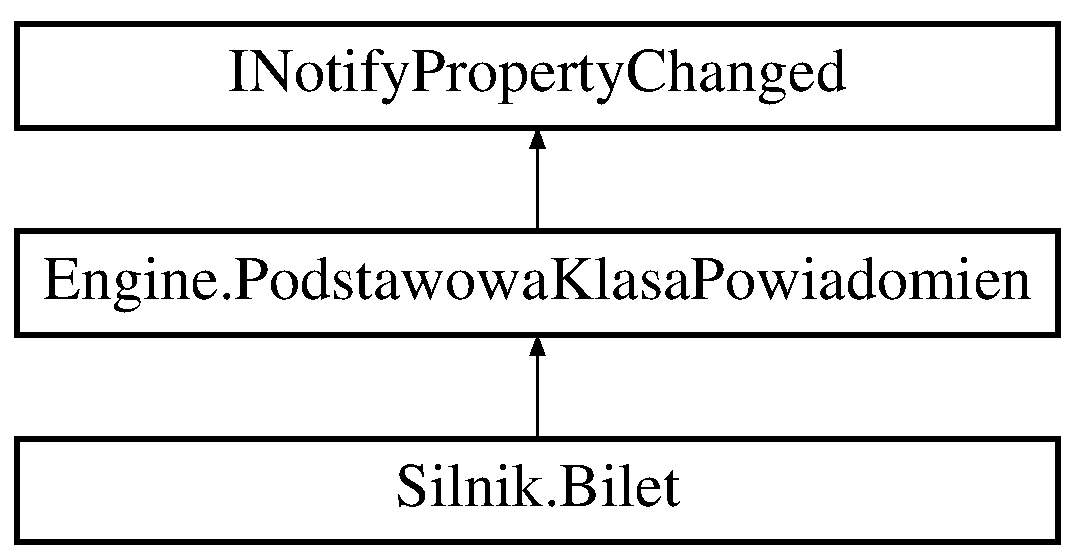
\includegraphics[height=3.000000cm]{class_silnik_1_1_bilet}
\end{center}
\end{figure}
\subsection*{Public Member Functions}
\begin{DoxyCompactItemize}
\item 
\mbox{\hyperlink{class_silnik_1_1_bilet_ab746139c19ca9a3ba4214e2edcca628a}{Bilet}} (\mbox{\hyperlink{class_silnik_1_1_klient}{Klient}} klient, int cena, int \mbox{\hyperlink{class_silnik_1_1_bilet_a44f01e9fea5fc9d9942a901df1854f61}{ID}})
\begin{DoxyCompactList}\small\item\em Initializes a new instance of the \mbox{\hyperlink{class_silnik_1_1_bilet}{Bilet}} class.\end{DoxyCompactList}\end{DoxyCompactItemize}
\subsection*{Properties}
\begin{DoxyCompactItemize}
\item 
int \mbox{\hyperlink{class_silnik_1_1_bilet_a44f01e9fea5fc9d9942a901df1854f61}{ID}}\hspace{0.3cm}{\ttfamily  \mbox{[}get, set\mbox{]}}
\begin{DoxyCompactList}\small\item\em Gets and sets id \end{DoxyCompactList}\item 
int \mbox{\hyperlink{class_silnik_1_1_bilet_ac9248d01d2d25b69868d614c3d98b814}{Cena}}\hspace{0.3cm}{\ttfamily  \mbox{[}get, set\mbox{]}}
\begin{DoxyCompactList}\small\item\em Gets and sets Cena \end{DoxyCompactList}\item 
\mbox{\hyperlink{class_silnik_1_1_klient}{Klient}} \mbox{\hyperlink{class_silnik_1_1_bilet_a04776d4ea2042538d57da9f3d35f3703}{Klient}}\hspace{0.3cm}{\ttfamily  \mbox{[}get, set\mbox{]}}
\begin{DoxyCompactList}\small\item\em Gets and sets \mbox{\hyperlink{class_silnik_1_1_klient}{Klient}} \end{DoxyCompactList}\end{DoxyCompactItemize}
\subsection*{Additional Inherited Members}


\subsection{Detailed Description}
The main \mbox{\hyperlink{class_silnik_1_1_bilet}{Bilet}} class. Represents ticket and it values. 



\subsection{Constructor \& Destructor Documentation}
\mbox{\Hypertarget{class_silnik_1_1_bilet_ab746139c19ca9a3ba4214e2edcca628a}\label{class_silnik_1_1_bilet_ab746139c19ca9a3ba4214e2edcca628a}} 
\index{Silnik\+::\+Bilet@{Silnik\+::\+Bilet}!Bilet@{Bilet}}
\index{Bilet@{Bilet}!Silnik\+::\+Bilet@{Silnik\+::\+Bilet}}
\subsubsection{\texorpdfstring{Bilet()}{Bilet()}}
{\footnotesize\ttfamily Silnik.\+Bilet.\+Bilet (\begin{DoxyParamCaption}\item[{\mbox{\hyperlink{class_silnik_1_1_klient}{Klient}}}]{klient,  }\item[{int}]{cena,  }\item[{int}]{ID }\end{DoxyParamCaption})}



Initializes a new instance of the \mbox{\hyperlink{class_silnik_1_1_bilet}{Bilet}} class.



\subsection{Property Documentation}
\mbox{\Hypertarget{class_silnik_1_1_bilet_ac9248d01d2d25b69868d614c3d98b814}\label{class_silnik_1_1_bilet_ac9248d01d2d25b69868d614c3d98b814}} 
\index{Silnik\+::\+Bilet@{Silnik\+::\+Bilet}!Cena@{Cena}}
\index{Cena@{Cena}!Silnik\+::\+Bilet@{Silnik\+::\+Bilet}}
\subsubsection{\texorpdfstring{Cena}{Cena}}
{\footnotesize\ttfamily int Silnik.\+Bilet.\+Cena\hspace{0.3cm}{\ttfamily [get]}, {\ttfamily [set]}}



Gets and sets Cena 

\mbox{\Hypertarget{class_silnik_1_1_bilet_a44f01e9fea5fc9d9942a901df1854f61}\label{class_silnik_1_1_bilet_a44f01e9fea5fc9d9942a901df1854f61}} 
\index{Silnik\+::\+Bilet@{Silnik\+::\+Bilet}!ID@{ID}}
\index{ID@{ID}!Silnik\+::\+Bilet@{Silnik\+::\+Bilet}}
\subsubsection{\texorpdfstring{ID}{ID}}
{\footnotesize\ttfamily int Silnik.\+Bilet.\+ID\hspace{0.3cm}{\ttfamily [get]}, {\ttfamily [set]}}



Gets and sets id 

\mbox{\Hypertarget{class_silnik_1_1_bilet_a04776d4ea2042538d57da9f3d35f3703}\label{class_silnik_1_1_bilet_a04776d4ea2042538d57da9f3d35f3703}} 
\index{Silnik\+::\+Bilet@{Silnik\+::\+Bilet}!Klient@{Klient}}
\index{Klient@{Klient}!Silnik\+::\+Bilet@{Silnik\+::\+Bilet}}
\subsubsection{\texorpdfstring{Klient}{Klient}}
{\footnotesize\ttfamily \mbox{\hyperlink{class_silnik_1_1_klient}{Klient}} Silnik.\+Bilet.\+Klient\hspace{0.3cm}{\ttfamily [get]}, {\ttfamily [set]}}



Gets and sets \mbox{\hyperlink{class_silnik_1_1_klient}{Klient}} 



The documentation for this class was generated from the following file\+:\begin{DoxyCompactItemize}
\item 
C\+:/\+Users/\+H\+P/source/repos/\+Project-\/2-\/2018/\+Kasa/\+Silnik/\+Models/Bilet.\+cs\end{DoxyCompactItemize}

\hypertarget{class_silnik_1_1_klient}{}\section{Silnik.\+Klient Class Reference}
\label{class_silnik_1_1_klient}\index{Silnik.\+Klient@{Silnik.\+Klient}}


Main \mbox{\hyperlink{class_silnik_1_1_klient}{Klient}} class Represents base of clients representation.  


Inheritance diagram for Silnik.\+Klient\+:\begin{figure}[H]
\begin{center}
\leavevmode
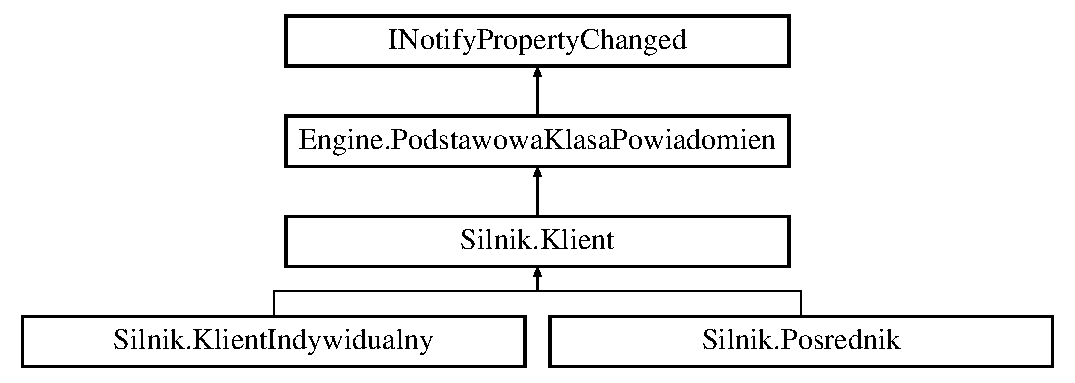
\includegraphics[height=4.000000cm]{class_silnik_1_1_klient}
\end{center}
\end{figure}
\subsection*{Properties}
\begin{DoxyCompactItemize}
\item 
int \mbox{\hyperlink{class_silnik_1_1_klient_ab301349e81e7495a1b07a1105d89e80b}{ID}}\hspace{0.3cm}{\ttfamily  \mbox{[}get, set\mbox{]}}
\begin{DoxyCompactList}\small\item\em Gets and sets ID \end{DoxyCompactList}\end{DoxyCompactItemize}
\subsection*{Additional Inherited Members}


\subsection{Detailed Description}
Main \mbox{\hyperlink{class_silnik_1_1_klient}{Klient}} class Represents base of clients representation. 



\subsection{Property Documentation}
\mbox{\Hypertarget{class_silnik_1_1_klient_ab301349e81e7495a1b07a1105d89e80b}\label{class_silnik_1_1_klient_ab301349e81e7495a1b07a1105d89e80b}} 
\index{Silnik\+::\+Klient@{Silnik\+::\+Klient}!ID@{ID}}
\index{ID@{ID}!Silnik\+::\+Klient@{Silnik\+::\+Klient}}
\subsubsection{\texorpdfstring{ID}{ID}}
{\footnotesize\ttfamily int Silnik.\+Klient.\+ID\hspace{0.3cm}{\ttfamily [get]}, {\ttfamily [set]}}



Gets and sets ID 



The documentation for this class was generated from the following file\+:\begin{DoxyCompactItemize}
\item 
C\+:/\+Users/\+H\+P/source/repos/\+Project-\/2-\/2018/\+Kasa/\+Silnik/\+Models/Klient.\+cs\end{DoxyCompactItemize}

\hypertarget{class_silnik_1_1_klient_indywidualny}{}\section{Silnik.\+Klient\+Indywidualny Class Reference}
\label{class_silnik_1_1_klient_indywidualny}\index{Silnik.\+Klient\+Indywidualny@{Silnik.\+Klient\+Indywidualny}}


\mbox{\hyperlink{class_silnik_1_1_klient}{Klient}} class Represents individual clients.  


Inheritance diagram for Silnik.\+Klient\+Indywidualny\+:\begin{figure}[H]
\begin{center}
\leavevmode
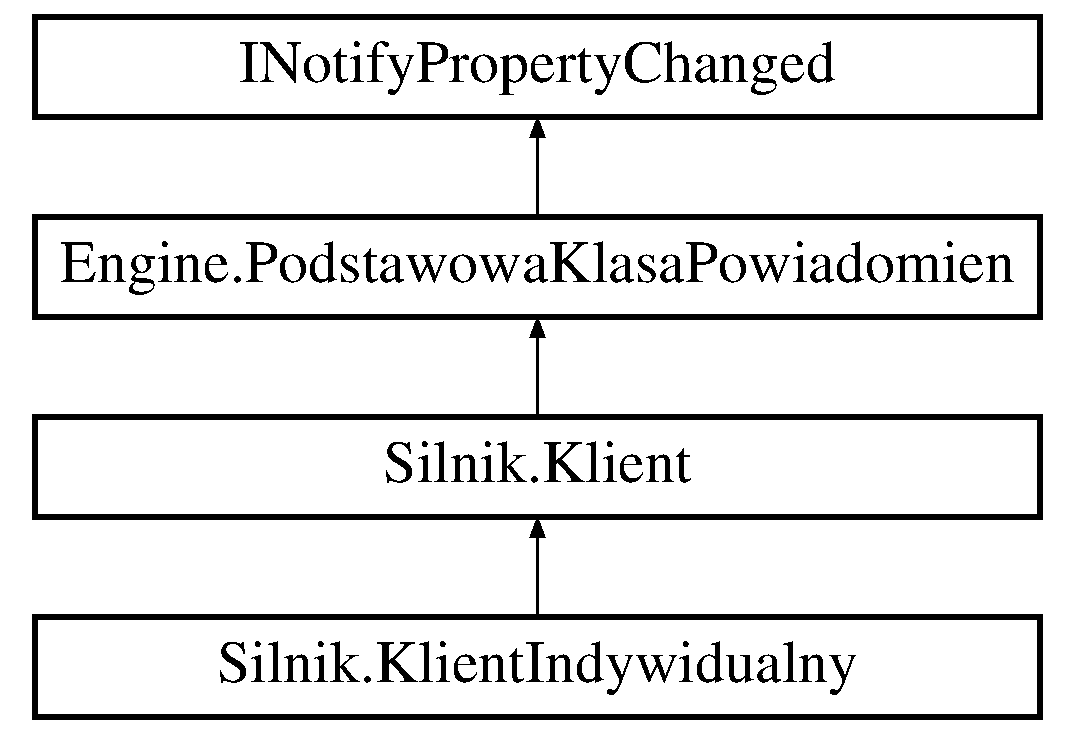
\includegraphics[height=4.000000cm]{class_silnik_1_1_klient_indywidualny}
\end{center}
\end{figure}
\subsection*{Public Member Functions}
\begin{DoxyCompactItemize}
\item 
\mbox{\hyperlink{class_silnik_1_1_klient_indywidualny_aad71a96b2d0b01f88f7a4f409f43f28b}{Klient\+Indywidualny}} (String imie, String nazwisko)
\begin{DoxyCompactList}\small\item\em Initializes a new instance of the \mbox{\hyperlink{class_silnik_1_1_klient_indywidualny}{Klient\+Indywidualny}} class. \end{DoxyCompactList}\end{DoxyCompactItemize}
\subsection*{Properties}
\begin{DoxyCompactItemize}
\item 
String \mbox{\hyperlink{class_silnik_1_1_klient_indywidualny_a91475465ea4c5df8a30690dd5d7cee94}{Imie}}\hspace{0.3cm}{\ttfamily  \mbox{[}get, set\mbox{]}}
\begin{DoxyCompactList}\small\item\em Gets and sets Imie \end{DoxyCompactList}\item 
String \mbox{\hyperlink{class_silnik_1_1_klient_indywidualny_ab5a0bdb5ed8412c91aeccb2833996607}{Nazwisko}}\hspace{0.3cm}{\ttfamily  \mbox{[}get, set\mbox{]}}
\begin{DoxyCompactList}\small\item\em Gets and sets Nazwisko \end{DoxyCompactList}\end{DoxyCompactItemize}
\subsection*{Additional Inherited Members}


\subsection{Detailed Description}
\mbox{\hyperlink{class_silnik_1_1_klient}{Klient}} class Represents individual clients. 



\subsection{Constructor \& Destructor Documentation}
\mbox{\Hypertarget{class_silnik_1_1_klient_indywidualny_aad71a96b2d0b01f88f7a4f409f43f28b}\label{class_silnik_1_1_klient_indywidualny_aad71a96b2d0b01f88f7a4f409f43f28b}} 
\index{Silnik\+::\+Klient\+Indywidualny@{Silnik\+::\+Klient\+Indywidualny}!Klient\+Indywidualny@{Klient\+Indywidualny}}
\index{Klient\+Indywidualny@{Klient\+Indywidualny}!Silnik\+::\+Klient\+Indywidualny@{Silnik\+::\+Klient\+Indywidualny}}
\subsubsection{\texorpdfstring{Klient\+Indywidualny()}{KlientIndywidualny()}}
{\footnotesize\ttfamily Silnik.\+Klient\+Indywidualny.\+Klient\+Indywidualny (\begin{DoxyParamCaption}\item[{String}]{imie,  }\item[{String}]{nazwisko }\end{DoxyParamCaption})}



Initializes a new instance of the \mbox{\hyperlink{class_silnik_1_1_klient_indywidualny}{Klient\+Indywidualny}} class. 


\begin{DoxyParams}{Parameters}
{\em imie} & Name of person\\
\hline
{\em nazwisko} & Surname of person\\
\hline
\end{DoxyParams}


\subsection{Property Documentation}
\mbox{\Hypertarget{class_silnik_1_1_klient_indywidualny_a91475465ea4c5df8a30690dd5d7cee94}\label{class_silnik_1_1_klient_indywidualny_a91475465ea4c5df8a30690dd5d7cee94}} 
\index{Silnik\+::\+Klient\+Indywidualny@{Silnik\+::\+Klient\+Indywidualny}!Imie@{Imie}}
\index{Imie@{Imie}!Silnik\+::\+Klient\+Indywidualny@{Silnik\+::\+Klient\+Indywidualny}}
\subsubsection{\texorpdfstring{Imie}{Imie}}
{\footnotesize\ttfamily String Silnik.\+Klient\+Indywidualny.\+Imie\hspace{0.3cm}{\ttfamily [get]}, {\ttfamily [set]}}



Gets and sets Imie 

\mbox{\Hypertarget{class_silnik_1_1_klient_indywidualny_ab5a0bdb5ed8412c91aeccb2833996607}\label{class_silnik_1_1_klient_indywidualny_ab5a0bdb5ed8412c91aeccb2833996607}} 
\index{Silnik\+::\+Klient\+Indywidualny@{Silnik\+::\+Klient\+Indywidualny}!Nazwisko@{Nazwisko}}
\index{Nazwisko@{Nazwisko}!Silnik\+::\+Klient\+Indywidualny@{Silnik\+::\+Klient\+Indywidualny}}
\subsubsection{\texorpdfstring{Nazwisko}{Nazwisko}}
{\footnotesize\ttfamily String Silnik.\+Klient\+Indywidualny.\+Nazwisko\hspace{0.3cm}{\ttfamily [get]}, {\ttfamily [set]}}



Gets and sets Nazwisko 



The documentation for this class was generated from the following file\+:\begin{DoxyCompactItemize}
\item 
C\+:/\+Users/\+H\+P/source/repos/\+Project-\/2-\/2018/\+Kasa/\+Silnik/\+Models/Klient\+Indywidualny.\+cs\end{DoxyCompactItemize}

\hypertarget{class_silnik_1_1_lot}{}\section{Silnik.\+Lot Class Reference}
\label{class_silnik_1_1_lot}\index{Silnik.\+Lot@{Silnik.\+Lot}}


Base \mbox{\hyperlink{class_silnik_1_1_lot}{Lot}} class Represents flight.  


Inheritance diagram for Silnik.\+Lot\+:\begin{figure}[H]
\begin{center}
\leavevmode
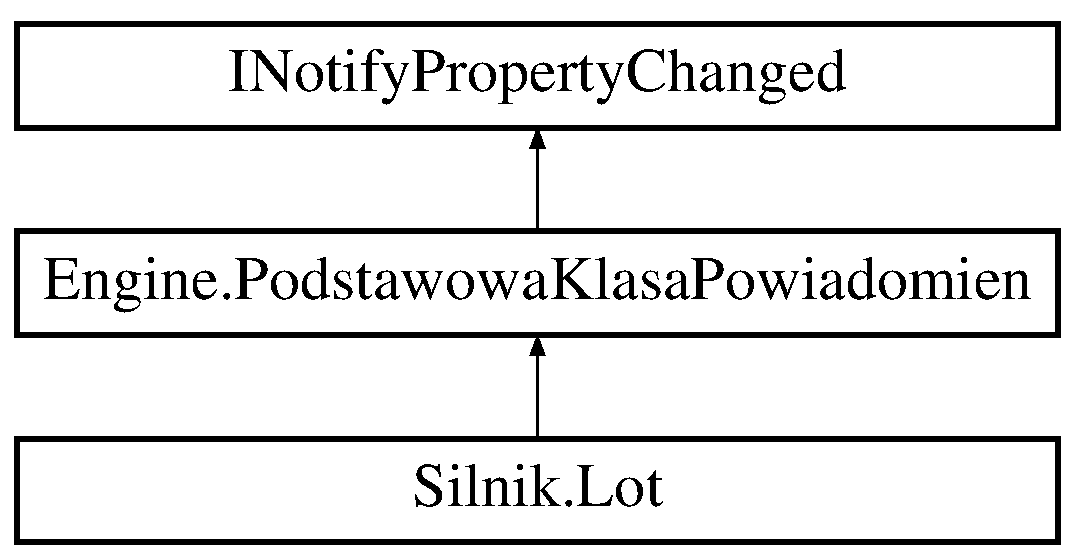
\includegraphics[height=3.000000cm]{class_silnik_1_1_lot}
\end{center}
\end{figure}
\subsection*{Public Member Functions}
\begin{DoxyCompactItemize}
\item 
\mbox{\hyperlink{class_silnik_1_1_lot_a6ff9543d81086a250b1c2517135e2499}{Lot}} (\mbox{\hyperlink{class_silnik_1_1_samolot}{Samolot}} samolot, \mbox{\hyperlink{class_silnik_1_1_trasa}{Trasa}} trasa, Date\+Time data\+Wylotu)
\begin{DoxyCompactList}\small\item\em Initializes a new instance of the \mbox{\hyperlink{class_silnik_1_1_lot}{Lot}} class. \end{DoxyCompactList}\item 
\mbox{\hyperlink{class_silnik_1_1_lot_a68a9f13aa20a3cfab653d70c227b70ca}{Lot}} (\mbox{\hyperlink{class_silnik_1_1_lot}{Lot}} lot)
\begin{DoxyCompactList}\small\item\em Initializes a new instance of the \mbox{\hyperlink{class_silnik_1_1_lot}{Lot}} class by coping paramethers of other. \end{DoxyCompactList}\item 
Boolean \mbox{\hyperlink{class_silnik_1_1_lot_a2623d91a3f8fb942ece1fc785465e5a5}{Rezerwuj\+Bilet}} (\mbox{\hyperlink{class_silnik_1_1_bilet}{Bilet}} bilet)
\begin{DoxyCompactList}\small\item\em Adds \mbox{\hyperlink{class_silnik_1_1_bilet}{Bilet}} to class. \end{DoxyCompactList}\item 
void \mbox{\hyperlink{class_silnik_1_1_lot_afc434618b4f20dd9aeb67db0adda5252}{Usun\+Bilet}} (\mbox{\hyperlink{class_silnik_1_1_bilet}{Bilet}} bilet)
\begin{DoxyCompactList}\small\item\em Removes \mbox{\hyperlink{class_silnik_1_1_bilet}{Bilet}} from class. \end{DoxyCompactList}\end{DoxyCompactItemize}
\subsection*{Public Attributes}
\begin{DoxyCompactItemize}
\item 
Observable\+Collection$<$ \mbox{\hyperlink{class_silnik_1_1_bilet}{Bilet}} $>$ \mbox{\hyperlink{class_silnik_1_1_lot_a3e02a16efd94bb1428ee6f3a34aacd8d}{bilety}}
\begin{DoxyCompactList}\small\item\em Stores Bilety\end{DoxyCompactList}\end{DoxyCompactItemize}
\subsection*{Properties}
\begin{DoxyCompactItemize}
\item 
int \mbox{\hyperlink{class_silnik_1_1_lot_afa780f21019d3396c86f1d0e67a0a02a}{ID}}\hspace{0.3cm}{\ttfamily  \mbox{[}get, set\mbox{]}}
\begin{DoxyCompactList}\small\item\em Gets and sets ID \end{DoxyCompactList}\item 
\mbox{\hyperlink{class_silnik_1_1_samolot}{Samolot}} \mbox{\hyperlink{class_silnik_1_1_lot_ad8823384ab258305bbc2dd1baee4eadd}{Samolot}}\hspace{0.3cm}{\ttfamily  \mbox{[}get, set\mbox{]}}
\begin{DoxyCompactList}\small\item\em Gets and sets \mbox{\hyperlink{class_silnik_1_1_samolot}{Samolot}} \end{DoxyCompactList}\item 
\mbox{\hyperlink{class_silnik_1_1_trasa}{Trasa}} \mbox{\hyperlink{class_silnik_1_1_lot_a665ef105afa7a29ee7870c720b762d6e}{Trasa}}\hspace{0.3cm}{\ttfamily  \mbox{[}get, set\mbox{]}}
\begin{DoxyCompactList}\small\item\em Gets and sets \mbox{\hyperlink{class_silnik_1_1_trasa}{Trasa}} \end{DoxyCompactList}\item 
Time\+Span \mbox{\hyperlink{class_silnik_1_1_lot_a7a4e0de2fff28c39b2f81a330235d1bd}{Czas\+Podruzy}}\hspace{0.3cm}{\ttfamily  \mbox{[}get, set\mbox{]}}
\begin{DoxyCompactList}\small\item\em Gets and sets Czas\+Podruzy \end{DoxyCompactList}\item 
Date\+Time \mbox{\hyperlink{class_silnik_1_1_lot_abff1662fa3776aab3d8889374bfb85f2}{Data\+Wylotu}}\hspace{0.3cm}{\ttfamily  \mbox{[}get, set\mbox{]}}
\begin{DoxyCompactList}\small\item\em Gets and sets Data\+Wylotu \end{DoxyCompactList}\item 
int \mbox{\hyperlink{class_silnik_1_1_lot_af5d78c458695021ff86158728209c31b}{Wolne\+Rezerwacje}}\hspace{0.3cm}{\ttfamily  \mbox{[}get, set\mbox{]}}
\begin{DoxyCompactList}\small\item\em Gets and sets Wolne\+Rezerwacje \end{DoxyCompactList}\item 
bool \mbox{\hyperlink{class_silnik_1_1_lot_a8246b195b85797bb116d4b1ac61c8082}{W\+Trakcie}}\hspace{0.3cm}{\ttfamily  \mbox{[}get, set\mbox{]}}
\begin{DoxyCompactList}\small\item\em Gets and sets W\+Trakcie \end{DoxyCompactList}\item 
Date\+Time \mbox{\hyperlink{class_silnik_1_1_lot_ac3b72a8fbb28b3dbbab0849caeec3aa9}{Data\+Przylotu}}\hspace{0.3cm}{\ttfamily  \mbox{[}get\mbox{]}}
\begin{DoxyCompactList}\small\item\em Gets automatic paramether Data\+Przylotu \end{DoxyCompactList}\item 
int \mbox{\hyperlink{class_silnik_1_1_lot_a9adba13eadf70435a63a5ecd9ed20cd2}{Rezerwacje}}\hspace{0.3cm}{\ttfamily  \mbox{[}get\mbox{]}}
\begin{DoxyCompactList}\small\item\em Gets automatic paramether Rezerwacje \end{DoxyCompactList}\end{DoxyCompactItemize}
\subsection*{Additional Inherited Members}


\subsection{Detailed Description}
Base \mbox{\hyperlink{class_silnik_1_1_lot}{Lot}} class Represents flight. 



\subsection{Constructor \& Destructor Documentation}
\mbox{\Hypertarget{class_silnik_1_1_lot_a6ff9543d81086a250b1c2517135e2499}\label{class_silnik_1_1_lot_a6ff9543d81086a250b1c2517135e2499}} 
\index{Silnik\+::\+Lot@{Silnik\+::\+Lot}!Lot@{Lot}}
\index{Lot@{Lot}!Silnik\+::\+Lot@{Silnik\+::\+Lot}}
\subsubsection{\texorpdfstring{Lot()}{Lot()}\hspace{0.1cm}{\footnotesize\ttfamily [1/2]}}
{\footnotesize\ttfamily Silnik.\+Lot.\+Lot (\begin{DoxyParamCaption}\item[{\mbox{\hyperlink{class_silnik_1_1_samolot}{Samolot}}}]{samolot,  }\item[{\mbox{\hyperlink{class_silnik_1_1_trasa}{Trasa}}}]{trasa,  }\item[{Date\+Time}]{data\+Wylotu }\end{DoxyParamCaption})}



Initializes a new instance of the \mbox{\hyperlink{class_silnik_1_1_lot}{Lot}} class. 


\begin{DoxyParams}{Parameters}
{\em data\+Wylotu} & Departure date.\\
\hline
{\em samolot} & Plane to be used.\\
\hline
{\em trasa} & Flight route to be taken.\\
\hline
\end{DoxyParams}
\mbox{\Hypertarget{class_silnik_1_1_lot_a68a9f13aa20a3cfab653d70c227b70ca}\label{class_silnik_1_1_lot_a68a9f13aa20a3cfab653d70c227b70ca}} 
\index{Silnik\+::\+Lot@{Silnik\+::\+Lot}!Lot@{Lot}}
\index{Lot@{Lot}!Silnik\+::\+Lot@{Silnik\+::\+Lot}}
\subsubsection{\texorpdfstring{Lot()}{Lot()}\hspace{0.1cm}{\footnotesize\ttfamily [2/2]}}
{\footnotesize\ttfamily Silnik.\+Lot.\+Lot (\begin{DoxyParamCaption}\item[{\mbox{\hyperlink{class_silnik_1_1_lot}{Lot}}}]{lot }\end{DoxyParamCaption})}



Initializes a new instance of the \mbox{\hyperlink{class_silnik_1_1_lot}{Lot}} class by coping paramethers of other. 


\begin{DoxyParams}{Parameters}
{\em lot} & Flight to be copied\\
\hline
\end{DoxyParams}


\subsection{Member Function Documentation}
\mbox{\Hypertarget{class_silnik_1_1_lot_a2623d91a3f8fb942ece1fc785465e5a5}\label{class_silnik_1_1_lot_a2623d91a3f8fb942ece1fc785465e5a5}} 
\index{Silnik\+::\+Lot@{Silnik\+::\+Lot}!Rezerwuj\+Bilet@{Rezerwuj\+Bilet}}
\index{Rezerwuj\+Bilet@{Rezerwuj\+Bilet}!Silnik\+::\+Lot@{Silnik\+::\+Lot}}
\subsubsection{\texorpdfstring{Rezerwuj\+Bilet()}{RezerwujBilet()}}
{\footnotesize\ttfamily Boolean Silnik.\+Lot.\+Rezerwuj\+Bilet (\begin{DoxyParamCaption}\item[{\mbox{\hyperlink{class_silnik_1_1_bilet}{Bilet}}}]{bilet }\end{DoxyParamCaption})}



Adds \mbox{\hyperlink{class_silnik_1_1_bilet}{Bilet}} to class. 


\begin{DoxyParams}{Parameters}
{\em bilet} & Ticket to be added.\\
\hline
\end{DoxyParams}
\begin{DoxyReturn}{Returns}
{\ttfamily true} if bilet could be added; otherwise {\ttfamily false}.
\end{DoxyReturn}
\mbox{\Hypertarget{class_silnik_1_1_lot_afc434618b4f20dd9aeb67db0adda5252}\label{class_silnik_1_1_lot_afc434618b4f20dd9aeb67db0adda5252}} 
\index{Silnik\+::\+Lot@{Silnik\+::\+Lot}!Usun\+Bilet@{Usun\+Bilet}}
\index{Usun\+Bilet@{Usun\+Bilet}!Silnik\+::\+Lot@{Silnik\+::\+Lot}}
\subsubsection{\texorpdfstring{Usun\+Bilet()}{UsunBilet()}}
{\footnotesize\ttfamily void Silnik.\+Lot.\+Usun\+Bilet (\begin{DoxyParamCaption}\item[{\mbox{\hyperlink{class_silnik_1_1_bilet}{Bilet}}}]{bilet }\end{DoxyParamCaption})}



Removes \mbox{\hyperlink{class_silnik_1_1_bilet}{Bilet}} from class. 


\begin{DoxyParams}{Parameters}
{\em bilet} & Ticket to remove.\\
\hline
\end{DoxyParams}


\subsection{Member Data Documentation}
\mbox{\Hypertarget{class_silnik_1_1_lot_a3e02a16efd94bb1428ee6f3a34aacd8d}\label{class_silnik_1_1_lot_a3e02a16efd94bb1428ee6f3a34aacd8d}} 
\index{Silnik\+::\+Lot@{Silnik\+::\+Lot}!bilety@{bilety}}
\index{bilety@{bilety}!Silnik\+::\+Lot@{Silnik\+::\+Lot}}
\subsubsection{\texorpdfstring{bilety}{bilety}}
{\footnotesize\ttfamily Observable\+Collection$<$\mbox{\hyperlink{class_silnik_1_1_bilet}{Bilet}}$>$ Silnik.\+Lot.\+bilety}



Stores Bilety



\subsection{Property Documentation}
\mbox{\Hypertarget{class_silnik_1_1_lot_a7a4e0de2fff28c39b2f81a330235d1bd}\label{class_silnik_1_1_lot_a7a4e0de2fff28c39b2f81a330235d1bd}} 
\index{Silnik\+::\+Lot@{Silnik\+::\+Lot}!Czas\+Podruzy@{Czas\+Podruzy}}
\index{Czas\+Podruzy@{Czas\+Podruzy}!Silnik\+::\+Lot@{Silnik\+::\+Lot}}
\subsubsection{\texorpdfstring{Czas\+Podruzy}{CzasPodruzy}}
{\footnotesize\ttfamily Time\+Span Silnik.\+Lot.\+Czas\+Podruzy\hspace{0.3cm}{\ttfamily [get]}, {\ttfamily [set]}}



Gets and sets Czas\+Podruzy 

\mbox{\Hypertarget{class_silnik_1_1_lot_ac3b72a8fbb28b3dbbab0849caeec3aa9}\label{class_silnik_1_1_lot_ac3b72a8fbb28b3dbbab0849caeec3aa9}} 
\index{Silnik\+::\+Lot@{Silnik\+::\+Lot}!Data\+Przylotu@{Data\+Przylotu}}
\index{Data\+Przylotu@{Data\+Przylotu}!Silnik\+::\+Lot@{Silnik\+::\+Lot}}
\subsubsection{\texorpdfstring{Data\+Przylotu}{DataPrzylotu}}
{\footnotesize\ttfamily Date\+Time Silnik.\+Lot.\+Data\+Przylotu\hspace{0.3cm}{\ttfamily [get]}}



Gets automatic paramether Data\+Przylotu 

\mbox{\Hypertarget{class_silnik_1_1_lot_abff1662fa3776aab3d8889374bfb85f2}\label{class_silnik_1_1_lot_abff1662fa3776aab3d8889374bfb85f2}} 
\index{Silnik\+::\+Lot@{Silnik\+::\+Lot}!Data\+Wylotu@{Data\+Wylotu}}
\index{Data\+Wylotu@{Data\+Wylotu}!Silnik\+::\+Lot@{Silnik\+::\+Lot}}
\subsubsection{\texorpdfstring{Data\+Wylotu}{DataWylotu}}
{\footnotesize\ttfamily Date\+Time Silnik.\+Lot.\+Data\+Wylotu\hspace{0.3cm}{\ttfamily [get]}, {\ttfamily [set]}}



Gets and sets Data\+Wylotu 

\mbox{\Hypertarget{class_silnik_1_1_lot_afa780f21019d3396c86f1d0e67a0a02a}\label{class_silnik_1_1_lot_afa780f21019d3396c86f1d0e67a0a02a}} 
\index{Silnik\+::\+Lot@{Silnik\+::\+Lot}!ID@{ID}}
\index{ID@{ID}!Silnik\+::\+Lot@{Silnik\+::\+Lot}}
\subsubsection{\texorpdfstring{ID}{ID}}
{\footnotesize\ttfamily int Silnik.\+Lot.\+ID\hspace{0.3cm}{\ttfamily [get]}, {\ttfamily [set]}}



Gets and sets ID 

\mbox{\Hypertarget{class_silnik_1_1_lot_a9adba13eadf70435a63a5ecd9ed20cd2}\label{class_silnik_1_1_lot_a9adba13eadf70435a63a5ecd9ed20cd2}} 
\index{Silnik\+::\+Lot@{Silnik\+::\+Lot}!Rezerwacje@{Rezerwacje}}
\index{Rezerwacje@{Rezerwacje}!Silnik\+::\+Lot@{Silnik\+::\+Lot}}
\subsubsection{\texorpdfstring{Rezerwacje}{Rezerwacje}}
{\footnotesize\ttfamily int Silnik.\+Lot.\+Rezerwacje\hspace{0.3cm}{\ttfamily [get]}}



Gets automatic paramether Rezerwacje 

\mbox{\Hypertarget{class_silnik_1_1_lot_ad8823384ab258305bbc2dd1baee4eadd}\label{class_silnik_1_1_lot_ad8823384ab258305bbc2dd1baee4eadd}} 
\index{Silnik\+::\+Lot@{Silnik\+::\+Lot}!Samolot@{Samolot}}
\index{Samolot@{Samolot}!Silnik\+::\+Lot@{Silnik\+::\+Lot}}
\subsubsection{\texorpdfstring{Samolot}{Samolot}}
{\footnotesize\ttfamily \mbox{\hyperlink{class_silnik_1_1_samolot}{Samolot}} Silnik.\+Lot.\+Samolot\hspace{0.3cm}{\ttfamily [get]}, {\ttfamily [set]}}



Gets and sets \mbox{\hyperlink{class_silnik_1_1_samolot}{Samolot}} 

\mbox{\Hypertarget{class_silnik_1_1_lot_a665ef105afa7a29ee7870c720b762d6e}\label{class_silnik_1_1_lot_a665ef105afa7a29ee7870c720b762d6e}} 
\index{Silnik\+::\+Lot@{Silnik\+::\+Lot}!Trasa@{Trasa}}
\index{Trasa@{Trasa}!Silnik\+::\+Lot@{Silnik\+::\+Lot}}
\subsubsection{\texorpdfstring{Trasa}{Trasa}}
{\footnotesize\ttfamily \mbox{\hyperlink{class_silnik_1_1_trasa}{Trasa}} Silnik.\+Lot.\+Trasa\hspace{0.3cm}{\ttfamily [get]}, {\ttfamily [set]}}



Gets and sets \mbox{\hyperlink{class_silnik_1_1_trasa}{Trasa}} 

\mbox{\Hypertarget{class_silnik_1_1_lot_af5d78c458695021ff86158728209c31b}\label{class_silnik_1_1_lot_af5d78c458695021ff86158728209c31b}} 
\index{Silnik\+::\+Lot@{Silnik\+::\+Lot}!Wolne\+Rezerwacje@{Wolne\+Rezerwacje}}
\index{Wolne\+Rezerwacje@{Wolne\+Rezerwacje}!Silnik\+::\+Lot@{Silnik\+::\+Lot}}
\subsubsection{\texorpdfstring{Wolne\+Rezerwacje}{WolneRezerwacje}}
{\footnotesize\ttfamily int Silnik.\+Lot.\+Wolne\+Rezerwacje\hspace{0.3cm}{\ttfamily [get]}, {\ttfamily [set]}}



Gets and sets Wolne\+Rezerwacje 

\mbox{\Hypertarget{class_silnik_1_1_lot_a8246b195b85797bb116d4b1ac61c8082}\label{class_silnik_1_1_lot_a8246b195b85797bb116d4b1ac61c8082}} 
\index{Silnik\+::\+Lot@{Silnik\+::\+Lot}!W\+Trakcie@{W\+Trakcie}}
\index{W\+Trakcie@{W\+Trakcie}!Silnik\+::\+Lot@{Silnik\+::\+Lot}}
\subsubsection{\texorpdfstring{W\+Trakcie}{WTrakcie}}
{\footnotesize\ttfamily bool Silnik.\+Lot.\+W\+Trakcie\hspace{0.3cm}{\ttfamily [get]}, {\ttfamily [set]}}



Gets and sets W\+Trakcie 



The documentation for this class was generated from the following file\+:\begin{DoxyCompactItemize}
\item 
C\+:/\+Users/\+H\+P/source/repos/\+Project-\/2-\/2018/\+Kasa/\+Silnik/\+Models/Lot.\+cs\end{DoxyCompactItemize}

\hypertarget{class_silnik_1_1_lotnisko}{}\section{Silnik.\+Lotnisko Class Reference}
\label{class_silnik_1_1_lotnisko}\index{Silnik.\+Lotnisko@{Silnik.\+Lotnisko}}


Base \mbox{\hyperlink{class_silnik_1_1_lotnisko}{Lotnisko}} class Represents airport.  


Inheritance diagram for Silnik.\+Lotnisko\+:\begin{figure}[H]
\begin{center}
\leavevmode
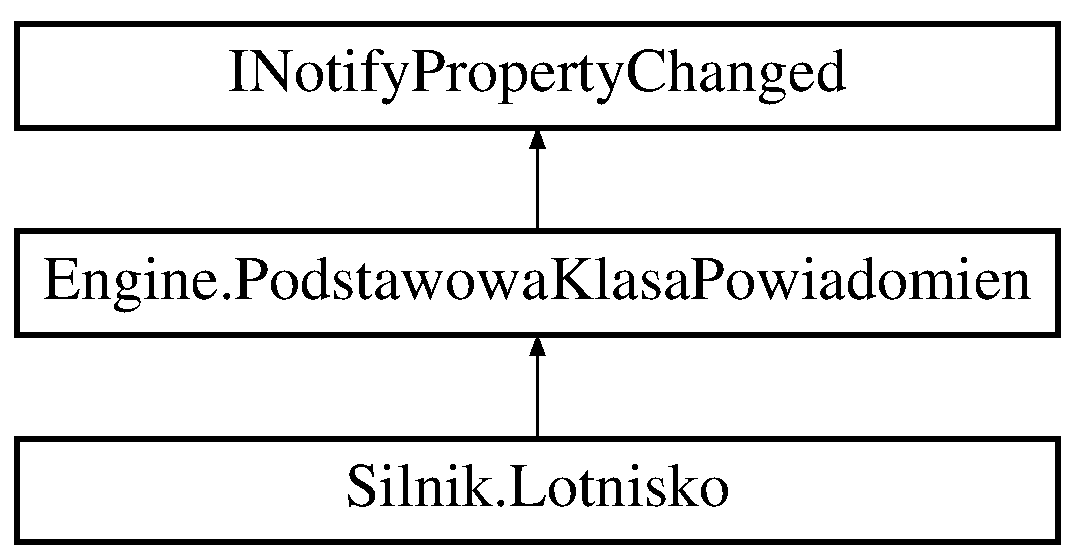
\includegraphics[height=3.000000cm]{class_silnik_1_1_lotnisko}
\end{center}
\end{figure}
\subsection*{Public Member Functions}
\begin{DoxyCompactItemize}
\item 
\mbox{\hyperlink{class_silnik_1_1_lotnisko_a42eff5febfea199bc94edab1693e801a}{Lotnisko}} (int id, String nazwa)
\begin{DoxyCompactList}\small\item\em Initializes a new instance of the \mbox{\hyperlink{class_silnik_1_1_lotnisko}{Lotnisko}} class. \end{DoxyCompactList}\item 
\mbox{\hyperlink{class_silnik_1_1_lotnisko_af5760fdf88ce17c44f0910b9cce9f1e7}{Lotnisko}} (\mbox{\hyperlink{class_silnik_1_1_lotnisko}{Lotnisko}} lotnisko)
\begin{DoxyCompactList}\small\item\em Initializes a new instance of the \mbox{\hyperlink{class_silnik_1_1_lotnisko}{Lotnisko}} class by copying paramethers of another. \end{DoxyCompactList}\end{DoxyCompactItemize}
\subsection*{Properties}
\begin{DoxyCompactItemize}
\item 
int \mbox{\hyperlink{class_silnik_1_1_lotnisko_a3b58935c64a4b7ebe2a3548b5f968583}{ID}}\hspace{0.3cm}{\ttfamily  \mbox{[}get, set\mbox{]}}
\begin{DoxyCompactList}\small\item\em Gets and sets ID \end{DoxyCompactList}\item 
String \mbox{\hyperlink{class_silnik_1_1_lotnisko_a9f92f264a5a3b2e5a8393fff6314d4ea}{Nazwa}}\hspace{0.3cm}{\ttfamily  \mbox{[}get\mbox{]}}
\begin{DoxyCompactList}\small\item\em Gets and sets Nazwa \end{DoxyCompactList}\end{DoxyCompactItemize}
\subsection*{Additional Inherited Members}


\subsection{Detailed Description}
Base \mbox{\hyperlink{class_silnik_1_1_lotnisko}{Lotnisko}} class Represents airport. 



\subsection{Constructor \& Destructor Documentation}
\mbox{\Hypertarget{class_silnik_1_1_lotnisko_a42eff5febfea199bc94edab1693e801a}\label{class_silnik_1_1_lotnisko_a42eff5febfea199bc94edab1693e801a}} 
\index{Silnik\+::\+Lotnisko@{Silnik\+::\+Lotnisko}!Lotnisko@{Lotnisko}}
\index{Lotnisko@{Lotnisko}!Silnik\+::\+Lotnisko@{Silnik\+::\+Lotnisko}}
\subsubsection{\texorpdfstring{Lotnisko()}{Lotnisko()}\hspace{0.1cm}{\footnotesize\ttfamily [1/2]}}
{\footnotesize\ttfamily Silnik.\+Lotnisko.\+Lotnisko (\begin{DoxyParamCaption}\item[{int}]{id,  }\item[{String}]{nazwa }\end{DoxyParamCaption})}



Initializes a new instance of the \mbox{\hyperlink{class_silnik_1_1_lotnisko}{Lotnisko}} class. 


\begin{DoxyParams}{Parameters}
{\em id} & Identificator of the airport\\
\hline
{\em nazwa} & Name of the airport\\
\hline
\end{DoxyParams}
\mbox{\Hypertarget{class_silnik_1_1_lotnisko_af5760fdf88ce17c44f0910b9cce9f1e7}\label{class_silnik_1_1_lotnisko_af5760fdf88ce17c44f0910b9cce9f1e7}} 
\index{Silnik\+::\+Lotnisko@{Silnik\+::\+Lotnisko}!Lotnisko@{Lotnisko}}
\index{Lotnisko@{Lotnisko}!Silnik\+::\+Lotnisko@{Silnik\+::\+Lotnisko}}
\subsubsection{\texorpdfstring{Lotnisko()}{Lotnisko()}\hspace{0.1cm}{\footnotesize\ttfamily [2/2]}}
{\footnotesize\ttfamily Silnik.\+Lotnisko.\+Lotnisko (\begin{DoxyParamCaption}\item[{\mbox{\hyperlink{class_silnik_1_1_lotnisko}{Lotnisko}}}]{lotnisko }\end{DoxyParamCaption})}



Initializes a new instance of the \mbox{\hyperlink{class_silnik_1_1_lotnisko}{Lotnisko}} class by copying paramethers of another. 


\begin{DoxyParams}{Parameters}
{\em lotnisko} & Airport to be copied.\\
\hline
\end{DoxyParams}


\subsection{Property Documentation}
\mbox{\Hypertarget{class_silnik_1_1_lotnisko_a3b58935c64a4b7ebe2a3548b5f968583}\label{class_silnik_1_1_lotnisko_a3b58935c64a4b7ebe2a3548b5f968583}} 
\index{Silnik\+::\+Lotnisko@{Silnik\+::\+Lotnisko}!ID@{ID}}
\index{ID@{ID}!Silnik\+::\+Lotnisko@{Silnik\+::\+Lotnisko}}
\subsubsection{\texorpdfstring{ID}{ID}}
{\footnotesize\ttfamily int Silnik.\+Lotnisko.\+ID\hspace{0.3cm}{\ttfamily [get]}, {\ttfamily [set]}}



Gets and sets ID 

\mbox{\Hypertarget{class_silnik_1_1_lotnisko_a9f92f264a5a3b2e5a8393fff6314d4ea}\label{class_silnik_1_1_lotnisko_a9f92f264a5a3b2e5a8393fff6314d4ea}} 
\index{Silnik\+::\+Lotnisko@{Silnik\+::\+Lotnisko}!Nazwa@{Nazwa}}
\index{Nazwa@{Nazwa}!Silnik\+::\+Lotnisko@{Silnik\+::\+Lotnisko}}
\subsubsection{\texorpdfstring{Nazwa}{Nazwa}}
{\footnotesize\ttfamily String Silnik.\+Lotnisko.\+Nazwa\hspace{0.3cm}{\ttfamily [get]}}



Gets and sets Nazwa 



The documentation for this class was generated from the following file\+:\begin{DoxyCompactItemize}
\item 
C\+:/\+Users/\+H\+P/source/repos/\+Project-\/2-\/2018/\+Kasa/\+Silnik/\+Models/Lotnisko.\+cs\end{DoxyCompactItemize}

\hypertarget{class_system_zarzadzania_1_1_main_window}{}\section{System\+Zarzadzania.\+Main\+Window Class Reference}
\label{class_system_zarzadzania_1_1_main_window}\index{System\+Zarzadzania.\+Main\+Window@{System\+Zarzadzania.\+Main\+Window}}


\mbox{\hyperlink{class_system_zarzadzania_1_1_main_window}{Main\+Window}}  


Inheritance diagram for System\+Zarzadzania.\+Main\+Window\+:\begin{figure}[H]
\begin{center}
\leavevmode
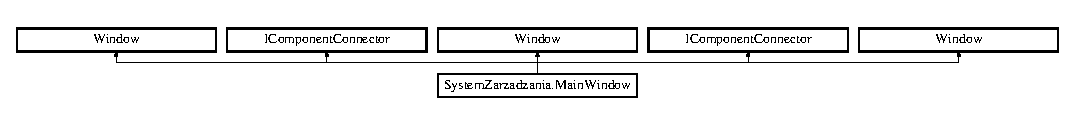
\includegraphics[height=1.082126cm]{class_system_zarzadzania_1_1_main_window}
\end{center}
\end{figure}
\subsection*{Public Member Functions}
\begin{DoxyCompactItemize}
\item 
\mbox{\Hypertarget{class_system_zarzadzania_1_1_main_window_a6814f7b2e20d09335a4aa767b9816263}\label{class_system_zarzadzania_1_1_main_window_a6814f7b2e20d09335a4aa767b9816263}} 
void {\bfseries main\+Serialize} ()
\item 
\mbox{\Hypertarget{class_system_zarzadzania_1_1_main_window_a74ba33358d5bc7f200f1e785f023e82b}\label{class_system_zarzadzania_1_1_main_window_a74ba33358d5bc7f200f1e785f023e82b}} 
void {\bfseries main\+Deserialize} ()
\item 
void \mbox{\hyperlink{class_system_zarzadzania_1_1_main_window_a6bf2b1fe2c258d549c389267f9053051}{Initialize\+Component}} ()
\begin{DoxyCompactList}\small\item\em Initialize\+Component \end{DoxyCompactList}\item 
void \mbox{\hyperlink{class_system_zarzadzania_1_1_main_window_a6bf2b1fe2c258d549c389267f9053051}{Initialize\+Component}} ()
\begin{DoxyCompactList}\small\item\em Initialize\+Component \end{DoxyCompactList}\end{DoxyCompactItemize}


\subsection{Detailed Description}
\mbox{\hyperlink{class_system_zarzadzania_1_1_main_window}{Main\+Window}} 



\subsection{Member Function Documentation}
\mbox{\Hypertarget{class_system_zarzadzania_1_1_main_window_a6bf2b1fe2c258d549c389267f9053051}\label{class_system_zarzadzania_1_1_main_window_a6bf2b1fe2c258d549c389267f9053051}} 
\index{System\+Zarzadzania\+::\+Main\+Window@{System\+Zarzadzania\+::\+Main\+Window}!Initialize\+Component@{Initialize\+Component}}
\index{Initialize\+Component@{Initialize\+Component}!System\+Zarzadzania\+::\+Main\+Window@{System\+Zarzadzania\+::\+Main\+Window}}
\subsubsection{\texorpdfstring{Initialize\+Component()}{InitializeComponent()}\hspace{0.1cm}{\footnotesize\ttfamily [1/2]}}
{\footnotesize\ttfamily void System\+Zarzadzania.\+Main\+Window.\+Initialize\+Component (\begin{DoxyParamCaption}{ }\end{DoxyParamCaption})}



Initialize\+Component 

\mbox{\Hypertarget{class_system_zarzadzania_1_1_main_window_a6bf2b1fe2c258d549c389267f9053051}\label{class_system_zarzadzania_1_1_main_window_a6bf2b1fe2c258d549c389267f9053051}} 
\index{System\+Zarzadzania\+::\+Main\+Window@{System\+Zarzadzania\+::\+Main\+Window}!Initialize\+Component@{Initialize\+Component}}
\index{Initialize\+Component@{Initialize\+Component}!System\+Zarzadzania\+::\+Main\+Window@{System\+Zarzadzania\+::\+Main\+Window}}
\subsubsection{\texorpdfstring{Initialize\+Component()}{InitializeComponent()}\hspace{0.1cm}{\footnotesize\ttfamily [2/2]}}
{\footnotesize\ttfamily void System\+Zarzadzania.\+Main\+Window.\+Initialize\+Component (\begin{DoxyParamCaption}{ }\end{DoxyParamCaption})}



Initialize\+Component 



The documentation for this class was generated from the following files\+:\begin{DoxyCompactItemize}
\item 
C\+:/\+Users/\+H\+P/source/repos/\+Project-\/2-\/2018/\+Kasa/\+System\+Zarzadzania/Main\+Window.\+xaml.\+cs\item 
C\+:/\+Users/\+H\+P/source/repos/\+Project-\/2-\/2018/\+Kasa/\+System\+Zarzadzania/obj/\+Debug/Main\+Window.\+g.\+cs\item 
C\+:/\+Users/\+H\+P/source/repos/\+Project-\/2-\/2018/\+Kasa/\+System\+Zarzadzania/obj/\+Debug/Main\+Window.\+g.\+i.\+cs\end{DoxyCompactItemize}

\hypertarget{class_engine_1_1_podstawowa_klasa_powiadomien}{}\section{Engine.\+Podstawowa\+Klasa\+Powiadomien Class Reference}
\label{class_engine_1_1_podstawowa_klasa_powiadomien}\index{Engine.\+Podstawowa\+Klasa\+Powiadomien@{Engine.\+Podstawowa\+Klasa\+Powiadomien}}
Inheritance diagram for Engine.\+Podstawowa\+Klasa\+Powiadomien\+:\begin{figure}[H]
\begin{center}
\leavevmode
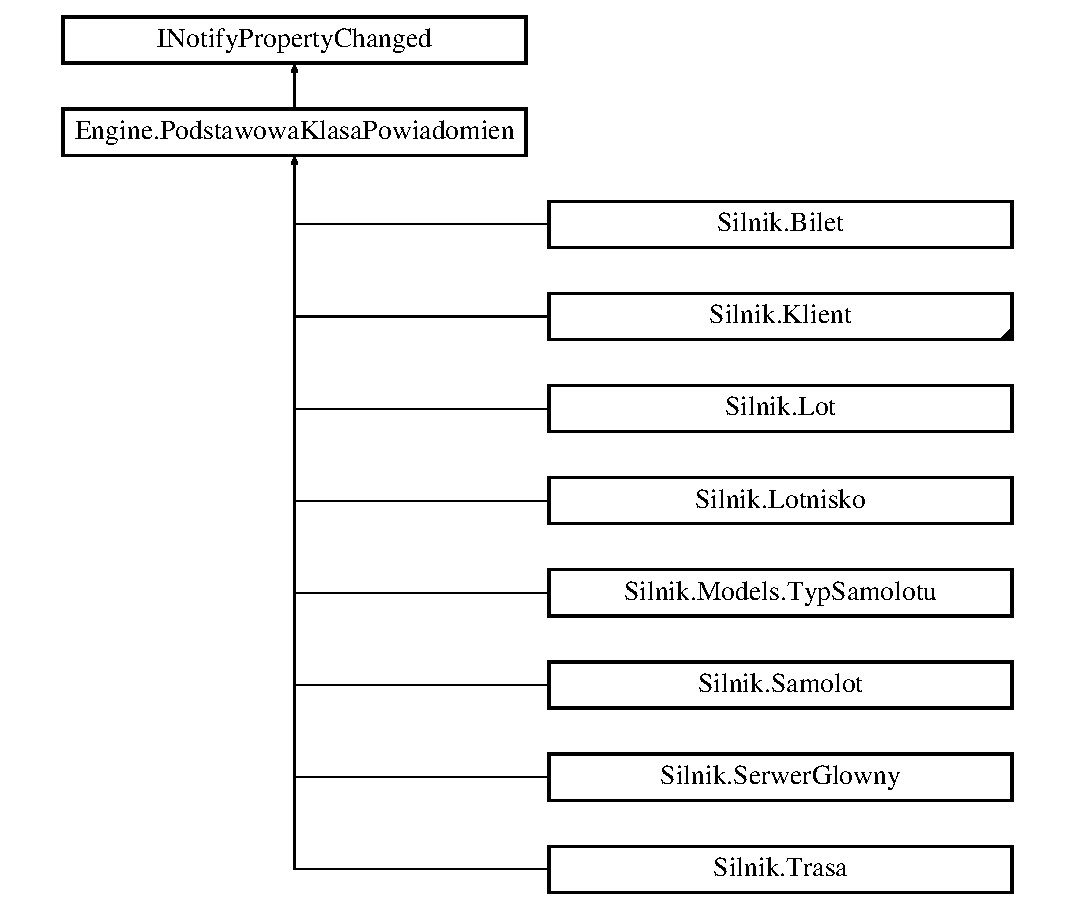
\includegraphics[height=10.000000cm]{class_engine_1_1_podstawowa_klasa_powiadomien}
\end{center}
\end{figure}
\subsection*{Protected Member Functions}
\begin{DoxyCompactItemize}
\item 
\mbox{\Hypertarget{class_engine_1_1_podstawowa_klasa_powiadomien_a1c3334a7504b249fe9c93f410c56fb7b}\label{class_engine_1_1_podstawowa_klasa_powiadomien_a1c3334a7504b249fe9c93f410c56fb7b}} 
void {\bfseries On\+Property\+Changed} (string name)
\end{DoxyCompactItemize}
\subsection*{Events}
\begin{DoxyCompactItemize}
\item 
\mbox{\Hypertarget{class_engine_1_1_podstawowa_klasa_powiadomien_a3b655c9a2008f6e9c68f60d6f7d243b4}\label{class_engine_1_1_podstawowa_klasa_powiadomien_a3b655c9a2008f6e9c68f60d6f7d243b4}} 
Property\+Changed\+Event\+Handler {\bfseries Property\+Changed}
\end{DoxyCompactItemize}


The documentation for this class was generated from the following file\+:\begin{DoxyCompactItemize}
\item 
C\+:/\+Users/\+H\+P/source/repos/\+Project-\/2-\/2018/\+Kasa/\+Silnik/Podstawowa\+Klasa\+Powiadomien.\+cs\end{DoxyCompactItemize}

\hypertarget{class_silnik_1_1_posrednik}{}\section{Silnik.\+Posrednik Class Reference}
\label{class_silnik_1_1_posrednik}\index{Silnik.\+Posrednik@{Silnik.\+Posrednik}}


\mbox{\hyperlink{class_silnik_1_1_posrednik}{Posrednik}} class Represents middleman.  


Inheritance diagram for Silnik.\+Posrednik\+:\begin{figure}[H]
\begin{center}
\leavevmode
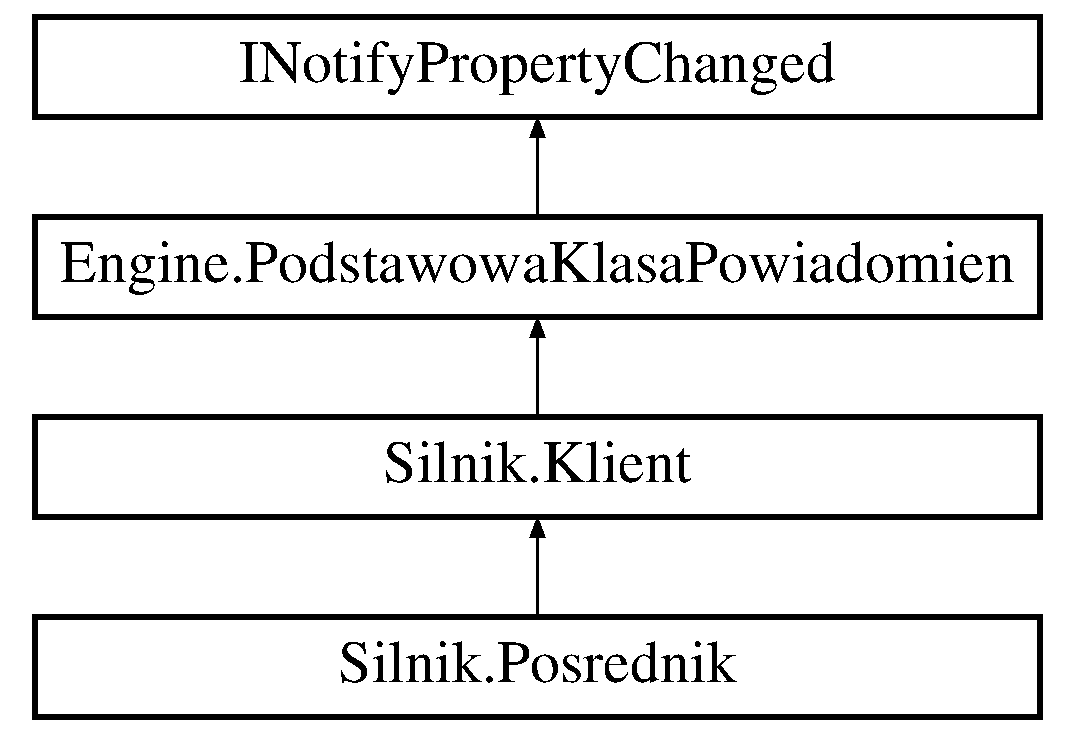
\includegraphics[height=4.000000cm]{class_silnik_1_1_posrednik}
\end{center}
\end{figure}
\subsection*{Public Member Functions}
\begin{DoxyCompactItemize}
\item 
\mbox{\hyperlink{class_silnik_1_1_posrednik_a55c7161a027803a4ca45a48466c13142}{Posrednik}} (String nazwa)
\begin{DoxyCompactList}\small\item\em Initializes a new instance of the \mbox{\hyperlink{class_silnik_1_1_posrednik}{Posrednik}} class. \end{DoxyCompactList}\end{DoxyCompactItemize}
\subsection*{Properties}
\begin{DoxyCompactItemize}
\item 
String \mbox{\hyperlink{class_silnik_1_1_posrednik_a2f7b267d89c092873db10e7928da53d7}{Nazwa}}\hspace{0.3cm}{\ttfamily  \mbox{[}get, set\mbox{]}}
\begin{DoxyCompactList}\small\item\em Gets and sets Nazwa \end{DoxyCompactList}\end{DoxyCompactItemize}
\subsection*{Additional Inherited Members}


\subsection{Detailed Description}
\mbox{\hyperlink{class_silnik_1_1_posrednik}{Posrednik}} class Represents middleman. 



\subsection{Constructor \& Destructor Documentation}
\mbox{\Hypertarget{class_silnik_1_1_posrednik_a55c7161a027803a4ca45a48466c13142}\label{class_silnik_1_1_posrednik_a55c7161a027803a4ca45a48466c13142}} 
\index{Silnik\+::\+Posrednik@{Silnik\+::\+Posrednik}!Posrednik@{Posrednik}}
\index{Posrednik@{Posrednik}!Silnik\+::\+Posrednik@{Silnik\+::\+Posrednik}}
\subsubsection{\texorpdfstring{Posrednik()}{Posrednik()}}
{\footnotesize\ttfamily Silnik.\+Posrednik.\+Posrednik (\begin{DoxyParamCaption}\item[{String}]{nazwa }\end{DoxyParamCaption})}



Initializes a new instance of the \mbox{\hyperlink{class_silnik_1_1_posrednik}{Posrednik}} class. 


\begin{DoxyParams}{Parameters}
{\em nazwa} & Name of middleman\\
\hline
\end{DoxyParams}


\subsection{Property Documentation}
\mbox{\Hypertarget{class_silnik_1_1_posrednik_a2f7b267d89c092873db10e7928da53d7}\label{class_silnik_1_1_posrednik_a2f7b267d89c092873db10e7928da53d7}} 
\index{Silnik\+::\+Posrednik@{Silnik\+::\+Posrednik}!Nazwa@{Nazwa}}
\index{Nazwa@{Nazwa}!Silnik\+::\+Posrednik@{Silnik\+::\+Posrednik}}
\subsubsection{\texorpdfstring{Nazwa}{Nazwa}}
{\footnotesize\ttfamily String Silnik.\+Posrednik.\+Nazwa\hspace{0.3cm}{\ttfamily [get]}, {\ttfamily [set]}}



Gets and sets Nazwa 



The documentation for this class was generated from the following file\+:\begin{DoxyCompactItemize}
\item 
C\+:/\+Users/\+H\+P/source/repos/\+Project-\/2-\/2018/\+Kasa/\+Silnik/\+Models/Posrednik.\+cs\end{DoxyCompactItemize}

\hypertarget{class_silnik_1_1_samolot}{}\section{Silnik.\+Samolot Class Reference}
\label{class_silnik_1_1_samolot}\index{Silnik.\+Samolot@{Silnik.\+Samolot}}
Inheritance diagram for Silnik.\+Samolot\+:\begin{figure}[H]
\begin{center}
\leavevmode
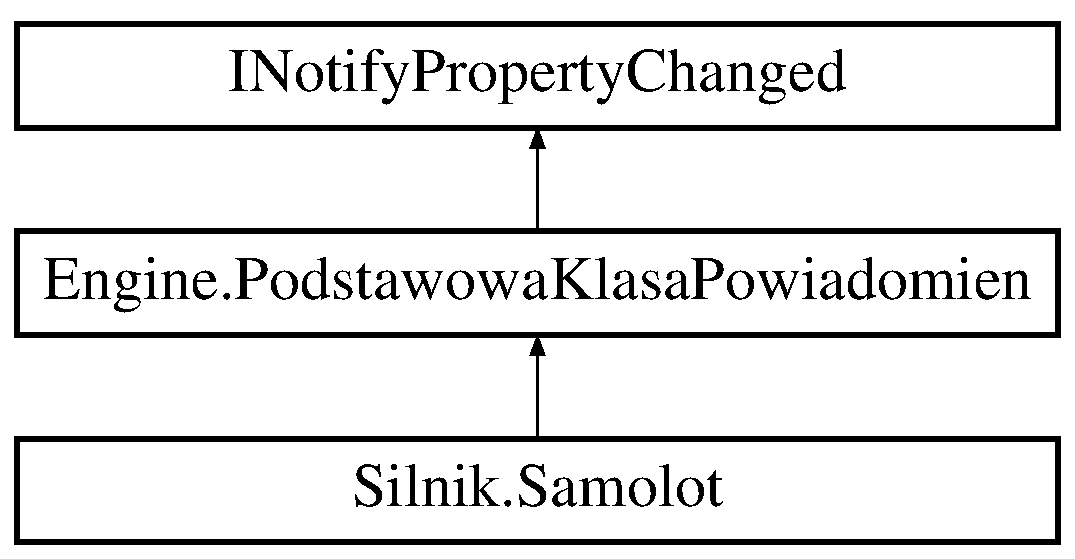
\includegraphics[height=3.000000cm]{class_silnik_1_1_samolot}
\end{center}
\end{figure}
\subsection*{Public Member Functions}
\begin{DoxyCompactItemize}
\item 
\mbox{\Hypertarget{class_silnik_1_1_samolot_aa11a612339f1e4d1ca48c0f0da3f3497}\label{class_silnik_1_1_samolot_aa11a612339f1e4d1ca48c0f0da3f3497}} 
{\bfseries Samolot} (String nazwa, int id, \mbox{\hyperlink{class_silnik_1_1_models_1_1_typ_samolotu}{Typ\+Samolotu}} typ, \mbox{\hyperlink{class_silnik_1_1_lotnisko}{Lotnisko}} lotnisko)
\item 
\mbox{\Hypertarget{class_silnik_1_1_samolot_a1eabd12a9871932843e841eb51dd3383}\label{class_silnik_1_1_samolot_a1eabd12a9871932843e841eb51dd3383}} 
{\bfseries Samolot} (\mbox{\hyperlink{class_silnik_1_1_samolot}{Samolot}} samolot)
\item 
\mbox{\Hypertarget{class_silnik_1_1_samolot_a2d01b94103ebc6a2741a435341673bf1}\label{class_silnik_1_1_samolot_a2d01b94103ebc6a2741a435341673bf1}} 
void {\bfseries Zmien\+Lotnisko} (\mbox{\hyperlink{class_silnik_1_1_lotnisko}{Lotnisko}} lotnisko)
\end{DoxyCompactItemize}
\subsection*{Properties}
\begin{DoxyCompactItemize}
\item 
\mbox{\Hypertarget{class_silnik_1_1_samolot_af9a4063dbb722f2db2009fd68cfd47c7}\label{class_silnik_1_1_samolot_af9a4063dbb722f2db2009fd68cfd47c7}} 
int {\bfseries ID}\hspace{0.3cm}{\ttfamily  \mbox{[}get, set\mbox{]}}
\item 
\mbox{\Hypertarget{class_silnik_1_1_samolot_aa1a2e910c38fe0c315f4f4dd5aba6da7}\label{class_silnik_1_1_samolot_aa1a2e910c38fe0c315f4f4dd5aba6da7}} 
String {\bfseries Nazwa}\hspace{0.3cm}{\ttfamily  \mbox{[}get\mbox{]}}
\item 
\mbox{\Hypertarget{class_silnik_1_1_samolot_a9eefea716beb59ccd0c824a7bd778d91}\label{class_silnik_1_1_samolot_a9eefea716beb59ccd0c824a7bd778d91}} 
\mbox{\hyperlink{class_silnik_1_1_models_1_1_typ_samolotu}{Typ\+Samolotu}} {\bfseries Typ\+Samolotu}\hspace{0.3cm}{\ttfamily  \mbox{[}get\mbox{]}}
\item 
\mbox{\Hypertarget{class_silnik_1_1_samolot_ac17b1d553d5f941bcdb141b4532cfef7}\label{class_silnik_1_1_samolot_ac17b1d553d5f941bcdb141b4532cfef7}} 
\mbox{\hyperlink{class_silnik_1_1_lotnisko}{Lotnisko}} {\bfseries Aktualne\+Lotnisko}\hspace{0.3cm}{\ttfamily  \mbox{[}get\mbox{]}}
\item 
\mbox{\Hypertarget{class_silnik_1_1_samolot_a0c75f071aa0cb7a9439144120fd3d4d1}\label{class_silnik_1_1_samolot_a0c75f071aa0cb7a9439144120fd3d4d1}} 
bool {\bfseries Przydzielony}\hspace{0.3cm}{\ttfamily  \mbox{[}get, set\mbox{]}}
\end{DoxyCompactItemize}
\subsection*{Additional Inherited Members}


The documentation for this class was generated from the following file\+:\begin{DoxyCompactItemize}
\item 
C\+:/\+Users/\+H\+P/source/repos/\+Project-\/2-\/2018/\+Kasa/\+Silnik/\+Models/Samolot.\+cs\end{DoxyCompactItemize}

\hypertarget{class_silnik_1_1_serwer_glowny}{}\section{Silnik.\+Serwer\+Glowny Class Reference}
\label{class_silnik_1_1_serwer_glowny}\index{Silnik.\+Serwer\+Glowny@{Silnik.\+Serwer\+Glowny}}
Inheritance diagram for Silnik.\+Serwer\+Glowny\+:\begin{figure}[H]
\begin{center}
\leavevmode
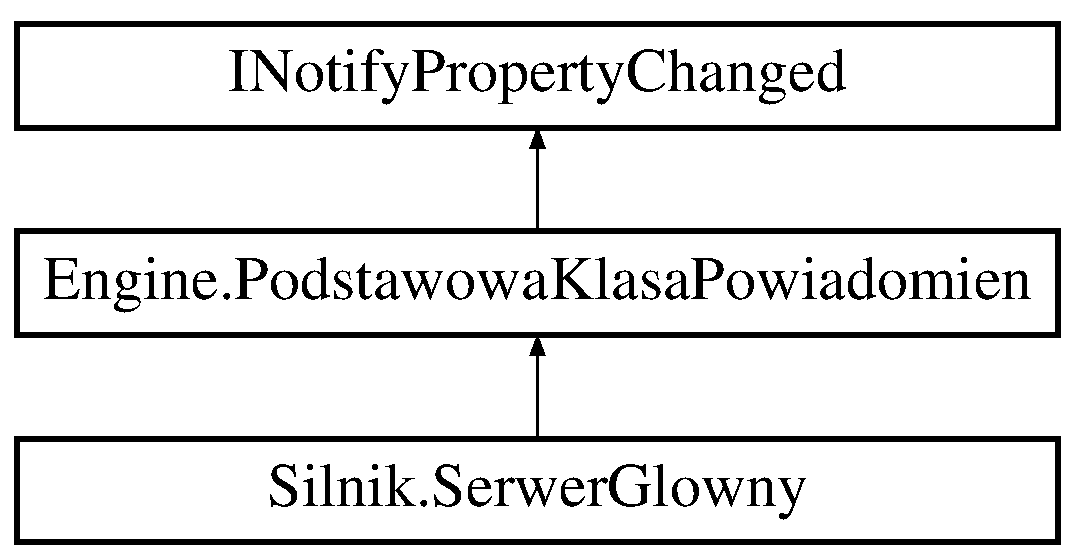
\includegraphics[height=3.000000cm]{class_silnik_1_1_serwer_glowny}
\end{center}
\end{figure}
\subsection*{Public Member Functions}
\begin{DoxyCompactItemize}
\item 
\mbox{\Hypertarget{class_silnik_1_1_serwer_glowny_a038bee5f4bf55a8b7c3f17f6f6fd2035}\label{class_silnik_1_1_serwer_glowny_a038bee5f4bf55a8b7c3f17f6f6fd2035}} 
void {\bfseries Dodaj\+Lotnisko} (\mbox{\hyperlink{class_silnik_1_1_lotnisko}{Lotnisko}} lotnisko)
\item 
\mbox{\Hypertarget{class_silnik_1_1_serwer_glowny_ac38b46d362c1752d3ec4e83b9cbbf6fe}\label{class_silnik_1_1_serwer_glowny_ac38b46d362c1752d3ec4e83b9cbbf6fe}} 
\mbox{\hyperlink{class_silnik_1_1_lotnisko}{Lotnisko}} {\bfseries Usun\+Lotnisko} (\mbox{\hyperlink{class_silnik_1_1_lotnisko}{Lotnisko}} lotnisko)
\item 
\mbox{\Hypertarget{class_silnik_1_1_serwer_glowny_a06a06b9eddac04e072a2e22f3bf9c529}\label{class_silnik_1_1_serwer_glowny_a06a06b9eddac04e072a2e22f3bf9c529}} 
void {\bfseries Dodaj\+Samolot} (\mbox{\hyperlink{class_silnik_1_1_samolot}{Samolot}} samolot)
\item 
\mbox{\Hypertarget{class_silnik_1_1_serwer_glowny_ac5eb09af8456690ad86dbe5c59c78009}\label{class_silnik_1_1_serwer_glowny_ac5eb09af8456690ad86dbe5c59c78009}} 
\mbox{\hyperlink{class_silnik_1_1_samolot}{Samolot}} {\bfseries Usun\+Samolot} (\mbox{\hyperlink{class_silnik_1_1_samolot}{Samolot}} samolot)
\item 
\mbox{\Hypertarget{class_silnik_1_1_serwer_glowny_a629fc578538155145b6e59799a532df0}\label{class_silnik_1_1_serwer_glowny_a629fc578538155145b6e59799a532df0}} 
void {\bfseries Dodaj\+Typ\+Samolotu} (\mbox{\hyperlink{class_silnik_1_1_models_1_1_typ_samolotu}{Typ\+Samolotu}} typ)
\item 
\mbox{\Hypertarget{class_silnik_1_1_serwer_glowny_a28abc6ed1ecc582ecdf336edc6cfcfc5}\label{class_silnik_1_1_serwer_glowny_a28abc6ed1ecc582ecdf336edc6cfcfc5}} 
\mbox{\hyperlink{class_silnik_1_1_models_1_1_typ_samolotu}{Typ\+Samolotu}} {\bfseries Usun\+Typ\+Samolotu} (\mbox{\hyperlink{class_silnik_1_1_models_1_1_typ_samolotu}{Typ\+Samolotu}} typ)
\item 
\mbox{\Hypertarget{class_silnik_1_1_serwer_glowny_afeabd8724c1c381de58880b1d1fb27f4}\label{class_silnik_1_1_serwer_glowny_afeabd8724c1c381de58880b1d1fb27f4}} 
void {\bfseries Dodaj\+Klienta} (\mbox{\hyperlink{class_silnik_1_1_klient}{Klient}} klient)
\item 
\mbox{\Hypertarget{class_silnik_1_1_serwer_glowny_aed68e1673af5c2fa2fad1527b368173b}\label{class_silnik_1_1_serwer_glowny_aed68e1673af5c2fa2fad1527b368173b}} 
\mbox{\hyperlink{class_silnik_1_1_klient}{Klient}} {\bfseries Usun\+Klienta} (\mbox{\hyperlink{class_silnik_1_1_klient}{Klient}} klient)
\item 
\mbox{\Hypertarget{class_silnik_1_1_serwer_glowny_a7c80e55b24f49993beef8fbda748fefb}\label{class_silnik_1_1_serwer_glowny_a7c80e55b24f49993beef8fbda748fefb}} 
void {\bfseries Usun\+Bilety} (\mbox{\hyperlink{class_silnik_1_1_klient}{Klient}} klient)
\item 
\mbox{\Hypertarget{class_silnik_1_1_serwer_glowny_a70356a55b8922f1034b75af18643717b}\label{class_silnik_1_1_serwer_glowny_a70356a55b8922f1034b75af18643717b}} 
void {\bfseries Dodaj\+Trase} (\mbox{\hyperlink{class_silnik_1_1_trasa}{Trasa}} trasa)
\item 
\mbox{\Hypertarget{class_silnik_1_1_serwer_glowny_a19e78c3461c71a0d45f894c3966968a8}\label{class_silnik_1_1_serwer_glowny_a19e78c3461c71a0d45f894c3966968a8}} 
\mbox{\hyperlink{class_silnik_1_1_trasa}{Trasa}} {\bfseries Usun\+Trase} (\mbox{\hyperlink{class_silnik_1_1_trasa}{Trasa}} trasa)
\item 
\mbox{\Hypertarget{class_silnik_1_1_serwer_glowny_afc4fbce7b7293acc01abd22a31a8f850}\label{class_silnik_1_1_serwer_glowny_afc4fbce7b7293acc01abd22a31a8f850}} 
void {\bfseries Dodaj\+Lot} (\mbox{\hyperlink{class_silnik_1_1_lot}{Lot}} lot)
\item 
\mbox{\Hypertarget{class_silnik_1_1_serwer_glowny_a921408ff90dd4874eb9dcd1f5ddc7952}\label{class_silnik_1_1_serwer_glowny_a921408ff90dd4874eb9dcd1f5ddc7952}} 
\mbox{\hyperlink{class_silnik_1_1_lot}{Lot}} {\bfseries Usun\+Lot} (\mbox{\hyperlink{class_silnik_1_1_lot}{Lot}} lot)
\item 
\mbox{\Hypertarget{class_silnik_1_1_serwer_glowny_a3407b4f0f0182f0f912572521f276af9}\label{class_silnik_1_1_serwer_glowny_a3407b4f0f0182f0f912572521f276af9}} 
void {\bfseries Generuj\+Loty} ()
\end{DoxyCompactItemize}
\subsection*{Public Attributes}
\begin{DoxyCompactItemize}
\item 
\mbox{\Hypertarget{class_silnik_1_1_serwer_glowny_a997b668c62a862c3ce11968c4a2f9ac4}\label{class_silnik_1_1_serwer_glowny_a997b668c62a862c3ce11968c4a2f9ac4}} 
Observable\+Collection$<$ \mbox{\hyperlink{class_silnik_1_1_lotnisko}{Lotnisko}} $>$ {\bfseries lotniska}
\item 
\mbox{\Hypertarget{class_silnik_1_1_serwer_glowny_a4ade6e5349d7077c5df7ca5be766be74}\label{class_silnik_1_1_serwer_glowny_a4ade6e5349d7077c5df7ca5be766be74}} 
Observable\+Collection$<$ \mbox{\hyperlink{class_silnik_1_1_models_1_1_typ_samolotu}{Typ\+Samolotu}} $>$ {\bfseries typy\+Samolotow}
\item 
\mbox{\Hypertarget{class_silnik_1_1_serwer_glowny_a6f254e519b4d4c940e93771a418ffe9b}\label{class_silnik_1_1_serwer_glowny_a6f254e519b4d4c940e93771a418ffe9b}} 
Observable\+Collection$<$ \mbox{\hyperlink{class_silnik_1_1_samolot}{Samolot}} $>$ {\bfseries samoloty}
\item 
\mbox{\Hypertarget{class_silnik_1_1_serwer_glowny_a30df3a2a391e6263c18b4b38a09c2537}\label{class_silnik_1_1_serwer_glowny_a30df3a2a391e6263c18b4b38a09c2537}} 
Observable\+Collection$<$ \mbox{\hyperlink{class_silnik_1_1_klient}{Klient}} $>$ {\bfseries klienci}
\item 
\mbox{\Hypertarget{class_silnik_1_1_serwer_glowny_a6c80036c19b7a40b06343367f6c2a700}\label{class_silnik_1_1_serwer_glowny_a6c80036c19b7a40b06343367f6c2a700}} 
Observable\+Collection$<$ \mbox{\hyperlink{class_silnik_1_1_trasa}{Trasa}} $>$ {\bfseries trasy}
\item 
\mbox{\Hypertarget{class_silnik_1_1_serwer_glowny_af876b3228f868008265515c158934f6a}\label{class_silnik_1_1_serwer_glowny_af876b3228f868008265515c158934f6a}} 
Observable\+Collection$<$ \mbox{\hyperlink{class_silnik_1_1_lot}{Lot}} $>$ {\bfseries loty}
\item 
\mbox{\Hypertarget{class_silnik_1_1_serwer_glowny_affd101ddff987ad456ed31691ea2197d}\label{class_silnik_1_1_serwer_glowny_affd101ddff987ad456ed31691ea2197d}} 
\mbox{\hyperlink{class_silnik_1_1_archiwum}{Archiwum}} {\bfseries archiwum}
\item 
\mbox{\Hypertarget{class_silnik_1_1_serwer_glowny_a85c0286cb27e56fd0ed6b60fd3070bea}\label{class_silnik_1_1_serwer_glowny_a85c0286cb27e56fd0ed6b60fd3070bea}} 
int {\bfseries lotniska\+ID}
\end{DoxyCompactItemize}
\subsection*{Additional Inherited Members}


The documentation for this class was generated from the following file\+:\begin{DoxyCompactItemize}
\item 
C\+:/\+Users/\+H\+P/source/repos/\+Project-\/2-\/2018/\+Kasa/\+Silnik/\+Models/Serwer\+Glowny.\+cs\end{DoxyCompactItemize}

\hypertarget{class_silnik_1_1_trasa}{}\section{Silnik.\+Trasa Class Reference}
\label{class_silnik_1_1_trasa}\index{Silnik.\+Trasa@{Silnik.\+Trasa}}
Inheritance diagram for Silnik.\+Trasa\+:\begin{figure}[H]
\begin{center}
\leavevmode
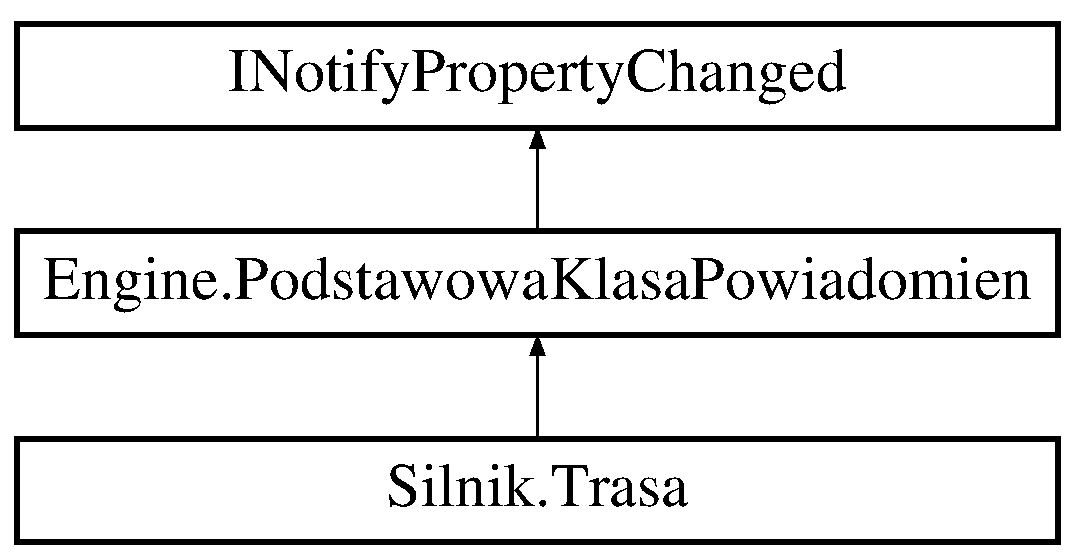
\includegraphics[height=3.000000cm]{class_silnik_1_1_trasa}
\end{center}
\end{figure}
\subsection*{Public Member Functions}
\begin{DoxyCompactItemize}
\item 
\mbox{\Hypertarget{class_silnik_1_1_trasa_aee3f0dcb8446e12b5c3fa3b227fae31e}\label{class_silnik_1_1_trasa_aee3f0dcb8446e12b5c3fa3b227fae31e}} 
{\bfseries Trasa} (int id, int odleglosc, int czestotliwosc, Date\+Time godzina\+Wylotu, \mbox{\hyperlink{class_silnik_1_1_lotnisko}{Lotnisko}} wylot, \mbox{\hyperlink{class_silnik_1_1_lotnisko}{Lotnisko}} destynacja)
\item 
\mbox{\Hypertarget{class_silnik_1_1_trasa_af49526eb2f9a0aa459a364ccd6f87eb8}\label{class_silnik_1_1_trasa_af49526eb2f9a0aa459a364ccd6f87eb8}} 
{\bfseries Trasa} (\mbox{\hyperlink{class_silnik_1_1_trasa}{Trasa}} trasa)
\end{DoxyCompactItemize}
\subsection*{Properties}
\begin{DoxyCompactItemize}
\item 
\mbox{\Hypertarget{class_silnik_1_1_trasa_a65bcfc1111e4909e0d690f411485bfd2}\label{class_silnik_1_1_trasa_a65bcfc1111e4909e0d690f411485bfd2}} 
int {\bfseries ID}\hspace{0.3cm}{\ttfamily  \mbox{[}get, set\mbox{]}}
\item 
\mbox{\Hypertarget{class_silnik_1_1_trasa_ae2d5aeb92c77808405469f00ff197ebe}\label{class_silnik_1_1_trasa_ae2d5aeb92c77808405469f00ff197ebe}} 
\mbox{\hyperlink{class_silnik_1_1_lotnisko}{Lotnisko}} {\bfseries Wylot}\hspace{0.3cm}{\ttfamily  \mbox{[}get, set\mbox{]}}
\item 
\mbox{\Hypertarget{class_silnik_1_1_trasa_acf60c1f4bcdad279d4c8e8c4b6683ee0}\label{class_silnik_1_1_trasa_acf60c1f4bcdad279d4c8e8c4b6683ee0}} 
\mbox{\hyperlink{class_silnik_1_1_lotnisko}{Lotnisko}} {\bfseries Destynacja}\hspace{0.3cm}{\ttfamily  \mbox{[}get, set\mbox{]}}
\item 
\mbox{\Hypertarget{class_silnik_1_1_trasa_a778d97e8538c64bbde98d6bbae1bd022}\label{class_silnik_1_1_trasa_a778d97e8538c64bbde98d6bbae1bd022}} 
Date\+Time {\bfseries Godzina\+Wylotu}\hspace{0.3cm}{\ttfamily  \mbox{[}get, set\mbox{]}}
\item 
\mbox{\Hypertarget{class_silnik_1_1_trasa_a6a8f71ffcf9cc3a914e4571d4528ab76}\label{class_silnik_1_1_trasa_a6a8f71ffcf9cc3a914e4571d4528ab76}} 
int {\bfseries Odleglosc}\hspace{0.3cm}{\ttfamily  \mbox{[}get, set\mbox{]}}
\item 
\mbox{\Hypertarget{class_silnik_1_1_trasa_a29c850dd0bd50113ea31d0b8b2811e36}\label{class_silnik_1_1_trasa_a29c850dd0bd50113ea31d0b8b2811e36}} 
int {\bfseries Czestotliwosc}\hspace{0.3cm}{\ttfamily  \mbox{[}get, set\mbox{]}}
\end{DoxyCompactItemize}
\subsection*{Additional Inherited Members}


The documentation for this class was generated from the following file\+:\begin{DoxyCompactItemize}
\item 
C\+:/\+Users/\+H\+P/source/repos/\+Project-\/2-\/2018/\+Kasa/\+Silnik/\+Models/Trasa.\+cs\end{DoxyCompactItemize}

\hypertarget{class_silnik_1_1_models_1_1_typ_samolotu}{}\section{Silnik.\+Models.\+Typ\+Samolotu Class Reference}
\label{class_silnik_1_1_models_1_1_typ_samolotu}\index{Silnik.\+Models.\+Typ\+Samolotu@{Silnik.\+Models.\+Typ\+Samolotu}}
Inheritance diagram for Silnik.\+Models.\+Typ\+Samolotu\+:\begin{figure}[H]
\begin{center}
\leavevmode
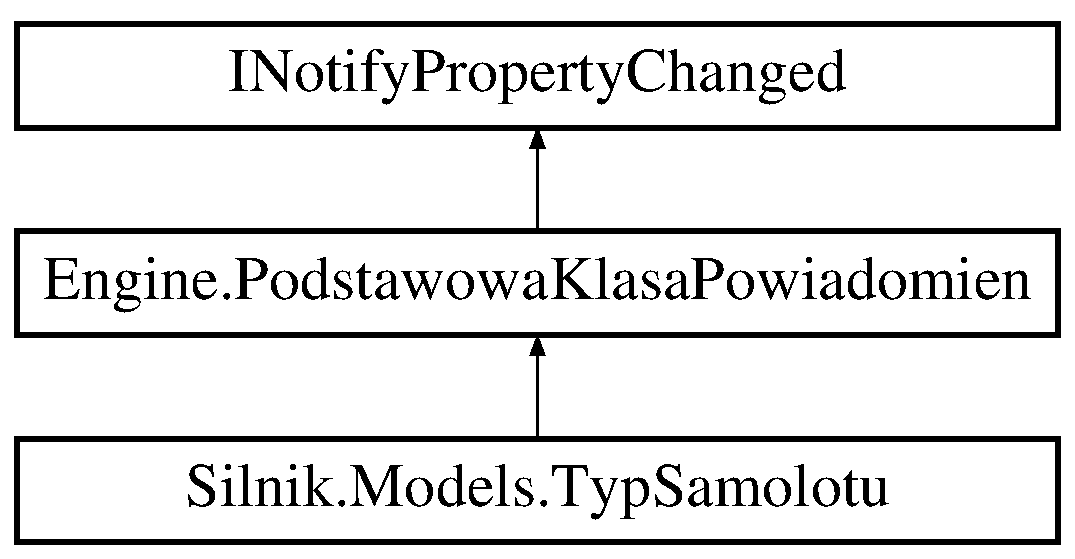
\includegraphics[height=3.000000cm]{class_silnik_1_1_models_1_1_typ_samolotu}
\end{center}
\end{figure}
\subsection*{Public Member Functions}
\begin{DoxyCompactItemize}
\item 
\mbox{\Hypertarget{class_silnik_1_1_models_1_1_typ_samolotu_ab338c993c75b09a7608efe91a6374b39}\label{class_silnik_1_1_models_1_1_typ_samolotu_ab338c993c75b09a7608efe91a6374b39}} 
{\bfseries Typ\+Samolotu} (int id, String nazwa, int zasieg, int ilosc\+Miejsc)
\item 
\mbox{\Hypertarget{class_silnik_1_1_models_1_1_typ_samolotu_a976ba346e05a686ec822ad0700053a79}\label{class_silnik_1_1_models_1_1_typ_samolotu_a976ba346e05a686ec822ad0700053a79}} 
{\bfseries Typ\+Samolotu} (\mbox{\hyperlink{class_silnik_1_1_models_1_1_typ_samolotu}{Typ\+Samolotu}} typ)
\end{DoxyCompactItemize}
\subsection*{Properties}
\begin{DoxyCompactItemize}
\item 
\mbox{\Hypertarget{class_silnik_1_1_models_1_1_typ_samolotu_a5160d3cdf6437ec96ba58ffc8260667d}\label{class_silnik_1_1_models_1_1_typ_samolotu_a5160d3cdf6437ec96ba58ffc8260667d}} 
int {\bfseries ID}\hspace{0.3cm}{\ttfamily  \mbox{[}get, set\mbox{]}}
\item 
\mbox{\Hypertarget{class_silnik_1_1_models_1_1_typ_samolotu_af60ab3d7f97de2fa381b5fe94a4aa47f}\label{class_silnik_1_1_models_1_1_typ_samolotu_af60ab3d7f97de2fa381b5fe94a4aa47f}} 
String {\bfseries Nazwa}\hspace{0.3cm}{\ttfamily  \mbox{[}get\mbox{]}}
\item 
\mbox{\Hypertarget{class_silnik_1_1_models_1_1_typ_samolotu_acbc91ae63d77cd7392e0a51fe3b30ad1}\label{class_silnik_1_1_models_1_1_typ_samolotu_acbc91ae63d77cd7392e0a51fe3b30ad1}} 
int {\bfseries Zasieg}\hspace{0.3cm}{\ttfamily  \mbox{[}get, set\mbox{]}}
\item 
\mbox{\Hypertarget{class_silnik_1_1_models_1_1_typ_samolotu_a1ff235a7c42697804e2266831e4ee0e7}\label{class_silnik_1_1_models_1_1_typ_samolotu_a1ff235a7c42697804e2266831e4ee0e7}} 
int {\bfseries Ilosc\+Miejsc}\hspace{0.3cm}{\ttfamily  \mbox{[}get, set\mbox{]}}
\end{DoxyCompactItemize}
\subsection*{Additional Inherited Members}


The documentation for this class was generated from the following file\+:\begin{DoxyCompactItemize}
\item 
C\+:/\+Users/\+H\+P/source/repos/\+Project-\/2-\/2018/\+Kasa/\+Silnik/\+Models/Typ\+Samolotu.\+cs\end{DoxyCompactItemize}

%--- End generated contents ---

% Index
\backmatter
\newpage
\phantomsection
\clearemptydoublepage
\addcontentsline{toc}{chapter}{Index}
\printindex

\end{document}
